\chapter{ĐỀ KIỂM TRA SỐ 1 – KHỐI ĐA DIỆN}
\setcounter{ex}{0}
\Opensolutionfile{ans}[ans/ans-2H1-5KT1-1]
\begin{ex}%Câu 1.%[Lương Như Quỳnh, TLDH4]%[2H1Y1-2]
	Cho khối đa diện đều $\{p;q\}$, chỉ số $p$ là
	\choice
	{\True Số các cạnh của mỗi mặt}
	{Số mặt của đa diện}
	{Số cạnh của đa diện}
	{Số đỉnh của đa diện}
	\loigiai{
	}
\end{ex}
\begin{ex}%Câu 2.%[Lương Như Quỳnh, TLDH4]%[2H1Y1-1]
	Có bao nhiêu khối đa diện đều?
	\choice
	{$4$}
	{\True $5$}
	{$3$}
	{$2$}
	\loigiai{
	}
\end{ex}
\begin{ex}%Câu 3.%[Lương Như Quỳnh, TLDH4]%[2H1Y1-1]
	Cho các hình sau
	\begin{center}
		\begin{tabular}{c c c c}
		\begin{tikzpicture}[join=round,line width=.6pt,scale=1]
		\path
		(0,0) coordinate (A) ++(45:1.6) coordinate (B) ++(0:2.8) coordinate (C) ++(-135:1.6) coordinate (D)
		(70:2.3) coordinate (A') ++(45:.8) coordinate (B') ++(0:1.4) coordinate (C') ++(-135:.8) coordinate (D')
		($(A')+(0,.8)$) coordinate (A'') ++(45:.8) coordinate (B'') ++(0:1.4) coordinate (C'') ++(-135:.8) coordinate (D'');
		\draw (A)--(D)--(C)--(C')--(C'')--(B'')--(A'')--(A')--cycle
			(A')--(D')--(C') (A'')--(D'')--(C'') (D)--(D')--(D'');
		\draw[dashed] (A)--(B)--(C) (A')--(B')--(C') (B)--(B')--(B'');
		\end{tikzpicture}
		&
		\begin{tikzpicture}[join=round,line width=.6pt,scale=1]
		\path
		(0,0) coordinate (A) ++(120:1.4) coordinate (B) ++(0:2.4) coordinate (C) ++(-60:1.4) coordinate (D)
		($(A)+(0,1.6)$) coordinate (A') ++(120:1.4) coordinate (B') ++(0:2.4) coordinate (C') ++(-60:1.4) coordinate (D')
		($(B')+(60:1.2)$) coordinate (A'') ++(0:2.4) coordinate (B'');
		\draw (A)--(A')--(D')--(D)--(A)--(B)--(B')-- (A') (D')--(C')--(B')--(A'')--(B'')--(C');
		\draw[dashed] (B)--(C)--(D) (C)--(C');
		\end{tikzpicture}
		&
		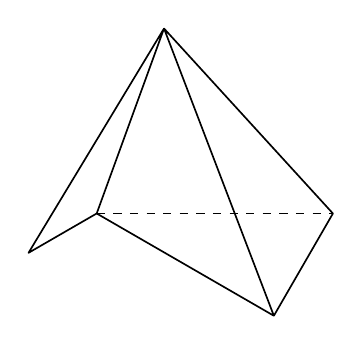
\begin{tikzpicture}[join=round,line width=.6pt,scale=1]
		\path
		(0,0) coordinate (A) ++(0:3) coordinate (B) ++(-120:1.5) coordinate (C)
		(-150:1) coordinate (D) (70:2.5) coordinate (E);
		\draw (A)--(D)--(E)--(A)--(C)--(B)--(E)--(C);
		\draw[dashed] (A)--(B);
		\end{tikzpicture}
		&
		\begin{tikzpicture}[join=round,line width=.6pt,scale=1]
		\path
		(0,0) coordinate (A) ++(120:1.4) coordinate (B) ++(0:2.4) coordinate (C) ++(-60:1.4) coordinate (D)
		($(A)+(0,1.6)$) coordinate (A') ++(120:1.4) coordinate (B') ++(0:2.4) coordinate (C') ++(-60:1.4) coordinate (D')
		($(B')!.25!(C')$) coordinate (M) ($(A')!.55!(D')$) coordinate (N)
		($(M)+(105:1)$) coordinate (A'') ++(.5,0) coordinate (B'') ($(N)-(M)+(B'')$) coordinate (C'')
		++(-.5,0) coordinate (D'');
		\coordinate (P) at (intersection of B'--C' and B''--C'');
		\draw (A)--(A')--(D')--(D)--(A)--(B)--(B')-- (A') (D')--(C')
		(A'')--(B'')--(C'')--(D'')--(A'')--(M)--(N)--(D'')  (N)--(C'') (B')--(M) (P)--(C');
		\draw[dashed] (B)--(C)--(D) (C)--(C') (B'')--(M)--(P);
		\end{tikzpicture}\\
		Hình 1&Hình 2&Hình 3&Hình 4 \vphantom{$ \dfrac{text}{den} $}
	\end{tabular}
	\end{center}
	Mỗi hình trên gồm một số hữu hạn đa giác phẳng (kể cả các điểm trong của nó), hình đa diện là
	\choice
	{\True Hình 1}
	{Hình 2}
	{Hình 3}
	{Hình 4}
	\loigiai{
	}
\end{ex}
\begin{ex}%Câu 4.%[Lương Như Quỳnh, TLDH4]%[2H1Y1-2]
	Hình đa diện trong hình vẽ sau có bao nhiêu mặt?
\begin{center}
			\begin{tikzpicture}[scale=1,x=1cm,y=1cm,line join=round,line cap=round]
			\tkzDefPoints{1/0/A,-1/-2/B,0.5/-2/C,2/-1.5/D,2.8/-0.4/E}
			\coordinate (A') at ($(A)+(0,.7)$);
			\coordinate (B') at ($(B)+(0,.7)$);
			\coordinate (M) at ($(B)!8/9!(C)$);
			\coordinate (C') at ($(M)+(-0.2,.7)$);
			\tkzDefPointBy[translation=from C to D](C')\tkzGetPoint{D'}
			\tkzDefPointBy[translation=from D to E](D')\tkzGetPoint{E'}
			\coordinate (A1) at ($(A')+(-0.4,.8)$);
			\coordinate (B1) at ($(B')+(.9,2.3)$);
			\coordinate (C1) at ($(C')+(.3,2.2)$);
			\coordinate (D1) at ($(D')+(-.5,1.8)$);
			\coordinate (E1) at ($(E')+(-1,1)$);
			\tkzDrawSegments(B,B' B',B1 C,C' C',C1 D,D' D',D1 E,E' E',E1 A1,B1 B1,C1 C1,D1 D1,E1 E1,A1 B',C' C',D' D',E' B,C C,D D,E)
			\tkzDrawSegments[dashed](A,A' A',A1 B,A  A,E B1,A1 A1,E1 B',A' A',E')
			\end{tikzpicture}
\end{center}
	\choice
	{$11$}
	{\True $12$}
	{$13$}
	{$14$}
	\loigiai{
	}
\end{ex}
\begin{ex}%Câu 5.%[Lương Như Quỳnh, TLDH4]%[2H1Y2-3]
	Số mặt phẳng đối xứng của hình tứ diện đều là
	\choice
	{$10$}
	{$8$}
	{\True $6$}
	{$4$}
	\loigiai{
	}
\end{ex}
\begin{ex}%Câu 6.%[Lương Như Quỳnh, TLDH4]%[2H1Y2-3]
Hình đa diện nào dưới đây {\bf không} có tâm đối xứng?
\begin{multicols}{4}	
\begin{center}
			\begin{tikzpicture}[scale=.42,x=1cm,y=1cm,line join=round,line cap=round]
			\tkzDefPoints{1/0/A,0/-1/B,2/-2.5/C,4/-2.5/D,5/-1.5/E,3/0/F}
			\coordinate (A') at ($(A)+(0,5)$);
			\coordinate (B') at ($(B)+(0,5)$);
			\coordinate (C') at ($(C)+(0,5)$);
			\coordinate (D') at ($(D)+(0,5)$);
			\coordinate (E') at ($(E)+(0,5)$);
			\coordinate (F') at ($(F)+(0,5)$);
		%	\tkzDrawPoints[fill = black](A,B,C,D,E,F,A',B',C',D',E',F')
			\tkzDrawSegments(B,C C,D D,E A',B' B',C' C',D' D',E' E',F' B,B' C,C' D,D' A',F' E,E')
			\tkzDrawSegments[dashed](A,A' E,E' A,B A,F F,E F,F')
			\end{tikzpicture}
\end{center}
\begin{center}
			\begin{tikzpicture}[scale=.3,x=1cm,y=1cm,line join=round,line cap=round]
			\tkzInit[xmin=-.5,ymin=-0.5,xmax=10.5,ymax=10.5]
			\tkzClip
			\tikzset{label style/.style={font=\footnotesize}}
			\tkzDefPoints{0/3/A,4/0/B,10/3/C,7/10/S}
			%\tkzDrawPoints[fill = black](S,A,B,C,D)
			\tkzDrawSegments(A,B B,C S,A S,B S,C)
			\tkzDrawSegments[dashed](A,C)
			\end{tikzpicture}
\end{center}		
\begin{center}
				\begin{tikzpicture}[scale=.6, line join=round, line cap=round]
				\tkzDefPoints{0/0/A,-1.3/-1.1/B,2/-1.1/C}
				\coordinate (D) at ($(A)+(C)-(B)$);
				\coordinate (A') at ($(A)+(0,3.3)$);
				\tkzDefPointsBy[translation=from A to A'](B,C,D){B'}{C'}{D'}
				\tkzDrawSegments(B,C A',B' A',D' B',C' C,D D,D' B',C' C',D' C,C' B,B')
				\tkzDrawSegments[dashed](A,B A,D A,A')
				%\tkzDrawPoints[fill=black,size=4](A,B,D,C,A',B',C',D')
				\end{tikzpicture}
\end{center}
				
\begin{center}
				\begin{tikzpicture}[scale=.6, line join=round, line cap=round]
				\tkzDefPoints{0/0/A,-1.5/-1.1/B,2/-1.1/C,.8/3/E,.8/-3/F}
				\coordinate (D) at ($(A)+(C)-(B)$);
				\tkzDrawSegments(B,C C,D E,B E,C E,D F,B F,C F,D)
				\tkzDrawSegments[dashed](A,B A,D E,A F,A)
				%\tkzDrawPoints[fill=black,size=4](A,B,D,C,E,F)
				\end{tikzpicture}
\end{center}
\end{multicols}
\choice
	{\True Tứ diện đều. }
	{Bát diện đều}
	{Hình lập phương. }
	{Lăng trụ lục giác đều. }
\loigiai{
}
\end{ex}

\begin{ex}%Câu 7.%[Lương Như Quỳnh, TLDH4]%[2H1Y2-2]
	Trong các mệnh đề sau mệnh đề nào {\bf sai}?
	\choice
	{Hình lăng trụ đều có cạnh bên vuông góc với đáy}
	{Hình lăng trụ đều có cạnh bên là các hình chữ nhật}
	{Hình lăng trụ đều có cạnh bên bằng đường cao của lăng trụ}
	{\True Hình lăng trụ đều có tất cả các cạnh đều bằng nhau}
	\loigiai{
	}
\end{ex}
\begin{ex}%Câu 8.%[Lương Như Quỳnh, TLDH4]%[2H1Y1-2]
	Số đỉnh của một hình bát diện đều là bao nhiêu?
	\choice
	{$10$}
	{$8$}
	{\True $6$}
	{$12$}
	\loigiai{
	}
\end{ex}
\begin{ex}%Câu 9.%[Lương Như Quỳnh, TLDH4]%[2H1B2-1]
	Cho hình lăng trụ $ABCD.A’B’C’D’$. Phát biểu nào sau đây là đúng?
	\choice
	{$ABCD.A’B’C’D’$ là hình hộp khi và chỉ khi $ABCD$ là hình chữ nhật}
	{Nếu $ABCD.A’B’C’D’$ là hình hộp thì $ABCD$ là hình chữ nhật}
	{Nếu $ABCD.A’B’C’D’$ là hình hộp thì $AA’\perp(ABCD)$}
	{\True $ABCD.A’B’C’D’$ là hình hộp khi và chỉ khi $ABCD$ là hình bình hành}
	\loigiai{
	}
\end{ex}
\begin{ex}%Câu 10.%[Lương Như Quỳnh, TLDH4]%[2H1B1-1]
	Tổng các góc của tất cả các mặt của khối đa diện đều loại $\{4;3\}$ là
	\choice
	{$4\pi$}
	{$8\pi$}
	{\True $12\pi$}
	{$10\pi$}
	\loigiai{
		Khối đa diện đều lọai $\{4;3\}$ là khối lập phương, gồm $6$ mặt là các hình vuông nên tổng các góc bằng $6\cdot 2\pi=12\pi$.}
\end{ex}
\begin{ex}%Câu 11.%[Lương Như Quỳnh, TLDH4]%[2H1B3-1]
	Tổng diện tích tất cả các mặt của hình tứ diện đều cạnh $a$ bằng
	\choice
	{$\dfrac{\sqrt{3}a^2}{2}$}
	{$2\sqrt{3}a^2$}
	{\True $\sqrt{3}a^2$}
	{$4\sqrt{3}a^2$}
	\loigiai{
Tứ diện đều có $4$ mặt là các tam giác đều cạnh $a$ nên tứ diện có tổng diện tích tất cả các mặt là $S=4\cdot\dfrac{\sqrt{3}a^2}{4}=\sqrt{3}a^2$.}
\end{ex}
\begin{ex}%Câu 12.%[Lương Như Quỳnh, TLDH4]%[2H1Y3-2]
	Tính thể của khối chóp có chiều cao $h$ và diện tích đáy là $B$ là
	\choice
	{$V=hB$}
	{\True $V=\dfrac{1}{3}hB$}
	{$V=3hB$}
	{$V=\dfrac{1}{6}hB$}
	\loigiai{
	}
\end{ex}
\begin{ex}%Câu 13.%[Lương Như Quỳnh, TLDH4]%[2H1B3-3]
	Cho tứ diện $MNPQ$. Gọi $I$; $J$; $K$ lần lượt là trung điểm của các cạnh $MN$; $MP$; $MQ$. Tính tỉ số thể tích $\dfrac{V_{MIJK}}{V_{MNPQ}}$.
	\choice
	{$\dfrac{1}{6}$}
	{\True $\dfrac{1}{8}$}
	{$\dfrac{1}{4}$}
	{$\dfrac{1}{3}$}
	\loigiai{
	\immini{
Do $I$; $J$; $K$ lần lượt nằm trên ba cạnh $MN$; $MP$; $MQ$ nên theo công thức tỉ số thể tích cho khối chóp tam giác ta có $$\dfrac{V_{MIJK}}{V_{MNPQ}}=\dfrac{MI}{MN}\cdot\dfrac{MJ}{MP}\cdot\dfrac{MK}{MQ} =\dfrac{1}{2}\cdot\dfrac{1}{2}\cdot\dfrac{1}{2}=\dfrac{1}{8}.$$}
		{
\begin{tikzpicture}[scale=0.6, line join = round, line cap = round]
\tikzset{label style/.style={font=\footnotesize}}
\tkzDefPoints{0/0/N,8/0/P,3/-3/Q}
\coordinate (M) at ($(N)+(4,5)$);
\coordinate (A) at ($(M)!1/2!(N)$);
\coordinate (B) at ($(M)!1/2!(Q)$);
\coordinate (C) at ($(M)!1/2!(P)$);
\tkzDrawPolygon(M,N,Q,P)
\tkzDrawSegments[dashed](N,P A,C)
\tkzDrawSegments(B,C A,B M,Q)
\tkzDrawPoints[fill=black](M,N,P,Q,A,B,C)
\tkzLabelPoints[above](M)
\tkzLabelPoints[left](A,N)
\tkzLabelPoints[right](C,P)
\tkzLabelPoints[below](Q)
\tkzLabelPoints[below right](B)
\end{tikzpicture}				
		}}
\end{ex}
\begin{ex}%Câu 14.%[Lương Như Quỳnh, TLDH4]%[2H1B3-2]
Cho hình chóp tứ giác $S.ABCD$ có đáy $ABCD$ là hình vuông cạnh $a$, $SA\perp(ABCD)$ và $SA=a\sqrt{6}$. Thể tích của khối chóp $S.ABCD$ bằng
	\choice
	{$\dfrac{a^3\sqrt{6}}{6}$}
	{$a^3\sqrt{6}$}
	{\True $\dfrac{a^3\sqrt{6}}{3}$}
	{$\dfrac{a^3\sqrt{6}}{2}$}
	\loigiai{
		$V=\dfrac{1}{3}\cdot SA\cdot S_{ABCD}=\dfrac{1}{3}\cdot a\sqrt{6}\cdot a^2=\dfrac{\sqrt{6}}{3}\cdot a^3$.}
\end{ex}
\begin{ex}%Câu 15.%[Lương Như Quỳnh, TLDH4]%[2H1B3-2]
Cho hình chóp tứ giác đều có tất cả các cạnh bằng nhau, đường cao của một mặt bên là $a\sqrt{3}$. Thể tích $V$ của khối chóp đó là
	\choice
	{$V=\dfrac{2\sqrt{2}}{3}a^3$}
	{\True $V=\dfrac{4\sqrt{2}}{3}a^3$}
	{$V=\dfrac{\sqrt{2}}{6}a^3$}
	{$V=\dfrac{\sqrt{2}}{9}a^3$}
	\loigiai{
	\immini{
		Ta có $SM=a\sqrt{3}$; $\Delta SCD$ đều nên $SC=CD=2a$.\\
		Suy ra $SO=\dfrac{AC}{2}=\dfrac{2a\sqrt{2}}{2}=a\sqrt{2}$.\\
		Vậy $V=\dfrac{1}{3}SO\cdot S_{ABCD}=\dfrac{1}{3}a\sqrt{2}\cdot 4a^2=\dfrac{4a^3\sqrt{2}}{3}$.}
		{
\begin{tikzpicture}[scale=0.55]
	\tkzDefPoints{0/0/O, -4/-1/B, 2/-1/C}
	\tkzDefPointBy[symmetry = center O](B)
	\tkzGetPoint{D}
	\tkzDefPointBy[symmetry = center O](C)
	\tkzGetPoint{A}
	\coordinate (M) at ($(C)!1/2!(D)$);
	\coordinate (N) at ($(B)!1/2!(C)$);
	\coordinate (S) at ($(O)+(0,6)$);
	\coordinate (P) at ($(A)!1/3!(N)$);
	\coordinate (Q) at ($(S)!2/3!(P)$);
	\tkzDrawSegments[dashed](S,A S,O A,C B,D O,M A,B A,D)
	\tkzDrawSegments(C,D S,B S,C B,C S,D S,M)
	\tkzLabelPoints[above](S)
	\tkzLabelPoints[below](O)
	\tkzLabelPoints[right](D)
	\tkzLabelPoints[below right](C,M)
	\tkzLabelPoints[below left](B)
	\tkzLabelPoints[left](A)
	\tkzDrawPoints[fill=black](A,B,C,D,S,O,M)
	\tkzMarkSegments[mark=|](M,D M,C)
	\end{tikzpicture}
		}}
\end{ex}
\begin{ex}%Câu 16.%[Lương Như Quỳnh, TLDH4]%[2H1B3-2]
	Cho khối chóp $S.ABC$ có đáy $ABC$ là tam giác cân tại $A$ với $BC=2a$, $\widehat{BAC}=120^{\circ}$, biết $SA\perp(ABC)$ và mặt $(SBC)$ hợp với đáy một góc $45^{\circ}$. Tính thể tích khối chóp $S.ABC$.
	\choice
	{$\dfrac{a^3}{3}$}
	{$a^3\sqrt{2}$}
	{$\dfrac{a^3}{2}$}
	{\True $\dfrac{a^3}{9}$}
	\loigiai{
		\immini{
		Gọi $M$ là trung điểm của $BC$.\\
		Ta có góc giữa $(SBC)$ và $(ABC)$ bằng $\widehat{SMA}=45^{\circ}$.\\
		$\Delta ABC$ cân tại $A$ nên $AM\perp BC$.\\
		$AM=\dfrac{BM}{\tan 60^{\circ}}=\dfrac{a}{\sqrt{3}}\Rightarrow SA=AM=\dfrac{a}{\sqrt{3}}$.\\
		$S_{ABC}=\dfrac{1}{2}AM\cdot BC=\dfrac{1}{2}\cdot\dfrac{a}{\sqrt{3}}\cdot 2a=\dfrac{a^2}{\sqrt{3}}$.\\
		$V_{S.ABC}=\dfrac{1}{3}SA\cdot S_{ABC}=\dfrac{1}{3}\dfrac{a}{\sqrt{3}}\cdot\dfrac{a^2}{\sqrt{3}}=\dfrac{a^3}{9}$.}
		{
\begin{tikzpicture}[scale=0.55, line join = round, line cap = round]
\tikzset{label style/.style={font=\footnotesize}}
\tkzDefPoints{0/0/A,7/0/B,-2.5/-3/C}
\coordinate (S) at ($(A)+(0,6.5)$);
\coordinate (M) at ($(C)!1/2!(B)$);
\tkzDrawPolygon(S,B,C)
\tkzDrawSegments(S,M)
\tkzDrawSegments[dashed](A,B A,C A,S A,M)
\tkzDrawPoints[fill=black](C,A,B,S)
\tkzLabelPoints[above](S)
\tkzLabelPoints[left](A,C)
\tkzLabelPoints[right](B)
\tkzLabelPoints[below right](M)
\tkzMarkAngle[size=.8](C,A,B)
\tkzLabelAngle[pos=1.2,dashed](C,A,B){\footnotesize $120^\circ$}
\tkzMarkAngle[size=.8](S,M,A)
\tkzLabelAngle[pos=1.3,dashed](S,M,A){\footnotesize $45^\circ$}
\end{tikzpicture}
		}		
		}
\end{ex}
\begin{ex}%Câu 17.%[Lương Như Quỳnh, TLDH4]%[2H1B3-2]
	Cho hình chóp $S.ABCD$ có đáy $ABCD$ là hình thang vuông tại $A$ và $B$, $AB=BC=a$, $SA=a$ và vuông góc với mặt phẳng $(ABCD)$. Khoảng cách từ $D$ đến mặt phẳng $(SAC)$ bằng $a\sqrt{2}$. Tính thể tích $V$ của khối chóp $S.ABCD$.
	\choice
	{$V=\dfrac{a^3\sqrt{3}}{4}$}
	{\True $V=\dfrac{a^3}{2}$}
	{$V=\dfrac{a^3\sqrt{3}}{6}$}
	{$V=\dfrac{a^3}{3}$}
	\loigiai{
\immini{
		Ta có $S_{ABCD}=S_{ABC}+S_{ADC}=\dfrac{a^2}{2}+\dfrac{1}{2}\cdot a\sqrt{2}\cdot a\sqrt{2}=\dfrac{3a^2}{2}$.\\
		Vậy $V_{ABCD}=\dfrac{1}{3}\cdot S_{ABCD}\cdot SA=\dfrac{1}{3}\cdot\dfrac{3a^2}{2}\cdot a=\dfrac{a^3}{2}$.}
		{
\begin{tikzpicture}[scale=0.55, line join = round, line cap = round]
\tikzset{label style/.style={font=\footnotesize}}
\tkzDefPoints{0/0/A,7/0/D,-2.5/-3/B, 4/-3/C}
\coordinate (S) at ($(A)+(0,6.5)$);
\coordinate (H) at ($(A)!4/5!(C)$);
\tkzDrawPolygon(S,B,C,D)
\tkzDrawSegments(S,C)
\tkzDrawSegments[dashed](A,B A,C A,S A,D D,H)
\tkzDrawPoints[fill=black](C,A,B,D,S,H)
\tkzLabelPoints[above](S)
\tkzLabelPoints[left](A,H,B)
\tkzLabelPoints[right](D)
\tkzLabelPoints[below right](C)
\end{tikzpicture}		
		}}
\end{ex}
\begin{ex}%Câu 18.%[Lương Như Quỳnh, TLDH4]%[2H1B3-2]
	Cho hình chóp $S.ABC$ có $SA=a$, tam giác $ABC$ đều, tam giác $SAB$ vuông cân tại $S$ và nằm trong mặt phẳng vuông góc với mặt phẳng đáy. Thể tích khối chóp $S.ABC$ bằng
	\choice
	{$\dfrac{\sqrt{6}a^3}{4}$}
	{$\dfrac{\sqrt{6}a^3}{24}$}
	{\True $\dfrac{\sqrt{6}a^3}{12}$}
	{$\dfrac{\sqrt{6}a^3}{8}$}
	\loigiai{
	\immini{
		Tam giác $SAB$ vuông cân tại $S$ và $SA=a$ nên $AB=a\sqrt{2}$.\\
		Gọi $M$ là trung điểm $AB$, ta có $SM\perp AB$ và $SM=\dfrac{AB}{2}=\dfrac{a\sqrt{2}}{2}$ ($SM$ là đường trung tuyến của tam giác $SAB$ vuông cân tại $S$).\\
		Mặt khác $(SAB)\perp(ABC)$, $SM\perp AB$ và $(SAB)\cap(ABC)=AB$ nên $SM\perp(ABC)$.\\
		Suy ra $SM$ là đường cao của hình chóp $S.ABC$ ứng với đáy là tam giác $ABC$.\\
		Thể tích khối chóp $S.ABC$ là $$V_{S.ABC}=\dfrac{1}{3}SM\cdot S_{\triangle ABC}=\dfrac{1}{3}\cdot\dfrac{a\sqrt{2}}{2}\cdot\dfrac{(a\sqrt{2})^2\sqrt{3}}{4} =\dfrac{a^3\sqrt{6}}{12}.$$}
		{
\begin{tikzpicture}[scale=0.55]
\tkzDefPoints{0/0/A,9/0/B,7/-3/C}
\coordinate (M) at ($(A)!1/2!(B)$);
\coordinate (S) at ($(M)+(0,6.5)$);
\tkzDrawPolygon(S,A,C,B)
\tkzDrawSegments(S,C)
\tkzDrawSegments[dashed](S,M A,B)
\tkzDrawPoints[fill=black](C,A,B,S,M)
\tkzLabelPoints[above](S)
\tkzLabelPoints[left](A)
\tkzLabelPoints[right](B)
\tkzLabelPoints[below](C,M)
\tkzDrawPoints[fill=black](A,B,C,S,M)
\tkzMarkSegments[mark=|](S,A S,B)
\tkzMarkRightAngle[size=.2](A,S,B)
\tkzMarkRightAngle[size=.2](S,M,A)
	\end{tikzpicture}		
		}}
\end{ex}
\begin{ex}%Câu 19.%[Lương Như Quỳnh, TLDH4]%[2H1B3-2]
	Một hình chóp tam giác đều có cạnh bên bằng $b$ và cạnh bên tạo với mặt phẳng đáy một góc $\alpha$. Thể tích của hình chóp đó là
	\choice
	{\True $\dfrac{\sqrt{3}}{4}b^3\cos^2\alpha\sin\alpha$}
	{$\dfrac{3}{4}b^3\sin^2\alpha\cos\alpha$}
	{$\dfrac{3}{4}b^3\cos^2\alpha\sin\alpha$}
	{$\dfrac{\sqrt{3}}{4}b^3\cos\alpha\sin\alpha$}
	\loigiai{		
		\immini{
		Gọi $M$ là trung điểm $BC$, $H$ là tâm tam giác $ABC$.\\
		Ta có $SH\perp(ABC)$.\\
		Xét tam giác $\Delta SHA$ vuông tại $H$, ta có\\
		$\heva{&SH=SA\sin\alpha=b\sin\alpha\\&AH=SA\cos\alpha=b\cos\alpha}$ \\
		Suy ra $ AM=\dfrac{3}{2}AH=\dfrac{3}{2}b\cos\alpha $.\\
		Mà $AM=\dfrac{AB\sqrt{3}}{2}\Rightarrow AB=\dfrac{2AM}{\sqrt{3}}=\sqrt{3}\cos\alpha$.\\
		$V_{SABC}=\dfrac{1}{3}\cdot SH\cdot S_{ABC}=\dfrac{1}{3}\cdot b\sin\alpha\cdot\dfrac{\sqrt{3}\left(\sqrt{3}b\cos\alpha\right)^2}{4}$.\\
		$V_{SABC}=\dfrac{\sqrt{3}}{4}b^3\cos^2\alpha\sin\alpha$.}
		{
\begin{tikzpicture}[scale=.8]
\tkzDefPoints{0/0/A, 4/-2/B, 6/0/C}
\coordinate (M) at ($(B)!.5!(C)$);
\coordinate (H) at ($(A)!.67!(M)$);
\coordinate (S) at ($(H)+(0,5)$);
\tkzDrawSegments[dashed](A,C S,H A,M)
\tkzDrawPolygon(S,B,C)
\tkzDrawSegments(S,A A,B S,M)
\tkzLabelPoints[left](A)
\tkzLabelPoints[right](C, M)
\tkzLabelPoints[below](B,H)
\tkzLabelPoints[above](S)
\tkzDrawPoints[fill=black](A,B,C,S,H,M)
\tkzMarkRightAngle[size=.2](M,H,S)
\tkzMarkRightAngle[size=.2](B,M,A)
\tkzMarkRightAngle[size=.2](S,M,C)
\tkzMarkSegments[mark=|](B,M M,C)
\tkzMarkAngle[size=.5](M,A,S)
\tkzLabelAngle[pos=1](S,A,M){$\alpha$}
\tkzLabelSegment[left,pos=0.5](S,A){$b$}
\end{tikzpicture}		
		}}
\end{ex}
\begin{ex}%Câu 20.%[Lương Như Quỳnh, TLDH4]%[2H1B3-3]
	Cho hình chóp $S.ABCD$. Gọi $M$, $N$, $P$, $Q$ lần lượt là trung điểm của $SA$, $SB$, $SC$, $SD$. Tỉ số thể tích của khối chóp $S.MNPQ$ và khối chóp $S.ABCD$ bằng
	\choice
	{\True $\dfrac{1}{8}$}
	{$\dfrac{1}{16}$}
	{$\dfrac{1}{4}$}
	{$\dfrac{1}{3}$}
	\loigiai{
	\immini{
		Tỉ số $\dfrac{V_{S.MNP}}{V_{S.ABC}}=\dfrac{SM}{SA}\cdot\dfrac{SN}{SB}\cdot\dfrac{SP}{SC}=\dfrac{1}{2}\cdot\dfrac{1}{2}\cdot\dfrac{1}{2}=\dfrac{1}{8}$.\\
		Tỉ số $\dfrac{V_{S.MPQ}}{V_{S.ACD}}=\dfrac{SM}{SA}\cdot\dfrac{SP}{SC}\cdot\dfrac{SQ}{SD}=\dfrac{1}{2}\cdot\dfrac{1}{2}\cdot\dfrac{1}{2}=\dfrac{1}{8}$. \\
		Suy ra\\
		$ V_{S.MNPQ}=V_{S.MNP}+V_{S.MPQ}=\dfrac{1}{8}V_{S.ABC}+\dfrac{1}{8}V_{S.ACD}=\dfrac{1}{8}V_{S.ABCD} $ \\
		Nên $ V_1=\dfrac{1}{8}V_2\Rightarrow\dfrac{V_1}{V_2}=\dfrac{1}{8} $.}
		{
\begin{tikzpicture}[scale=0.45, line join = round, line cap = round]
\tikzset{label style/.style={font=\footnotesize}}
\tkzDefPoints{0/0/A,8/0/D,-2.5/-3/B, 4/-4/C}
\coordinate (S) at ($(A)+(1,6.5)$);
\coordinate (M) at ($(A)!1/2!(S)$);
\coordinate (N) at ($(B)!1/2!(S)$);
\coordinate (P) at ($(S)!1/2!(C)$);
\coordinate (Q) at ($(S)!1/2!(D)$);
\tkzDrawPolygon(S,B,C,D)
\tkzDrawSegments(S,C N,P P,Q)
\tkzDrawSegments[dashed](A,B A,C A,S A,D M,N M,P M,Q)
\tkzDrawPoints[fill=black](C,A,B,D,S,M,N,P,Q)
\tkzLabelPoints[above](S)
\tkzLabelPoints[left](A,N)
\tkzLabelPoints[right](D,P,Q)
\tkzLabelPoints[below right](C)
\tkzLabelPoints[above right](M)
\tkzLabelPoints[below left](B)
\end{tikzpicture}				
		}}
\end{ex}
\begin{ex}%Câu 21.%[Lương Như Quỳnh, TLDH4]%[2H1K3-3]
	Cho hình chóp $S.ABCD$ có đáy $ABCD$ là hình chữ nhật. Mặt phẳng $(\alpha)$ đi qua $A$, $B$ và trung điểm $M$ của $SC$. Mặt phẳng $(\alpha)$ chia khối chóp đã cho thành hai phần có thể tích lần lượt là $V_1$, $V_2$ với $V_1<V_2$. Tính tỉ số $\dfrac{V_1}{V_2}$.
	\choice
	{$\dfrac{V_1}{V_2}=\dfrac{1}{4}$}
	{$\dfrac{V_1}{V_2}=\dfrac{3}{8}$}
	{$\dfrac{V_1}{V_2}=\dfrac{5}{8}$}
	{\True $\dfrac{V_1}{V_2}=\dfrac{3}{5}$}
	\loigiai{
	\immini{
		Kẻ $MN\parallel CD (N\in CD)$, suy ra $ABMN$ là thiết diện của khối chóp. \\
		Ta có $V_{S.ABMN}=V_{S.ABM}+V_{S.AMN}$.\\
		$\dfrac{V_{S.ABM}}{V_{S.ABC}}=\dfrac{SM}{SC}=\dfrac{1}{2}\Rightarrow V_{S.ABM}=\dfrac{1}{2}V_{S.ABC}=\dfrac{1}{4}V_{S.ABCD}$.\\
		$\dfrac{V_{S.AMN}}{V_{S.ACD}}=\dfrac{SM}{SC}\cdot\dfrac{SN}{SD}=\dfrac{1}{4}\Rightarrow V_{S.AMN}=\dfrac{1}{8}V_{S.ABCD}$.\\
		Do đó $V_{S.ABMN}=\dfrac{1}{4}V_{S.ABCD}+\dfrac{1}{8}V_{S.ABCD}=\dfrac{3}{8}V_{S.ABCD}$.\\
		Suy ra $V_{ABMNDC}=\dfrac{5}{8}V_{S.ABCD}$ nên $\dfrac{V_1}{V_2}=\dfrac{3}{5}$.}
		{
\begin{tikzpicture}[scale=0.55]
	\tkzDefPoints{0/0/O, -5/-1/B, 2/-1/C}
	\tkzDefPointBy[symmetry = center O](B)
	\tkzGetPoint{D}
	\tkzDefPointBy[symmetry = center O](C)
	\tkzGetPoint{A}
	\coordinate (M) at ($(S)!1/2!(C)$);
	\coordinate (N) at ($(S)!1/2!(D)$);
	\coordinate (S) at ($(A)+(-1,6.5)$);
	\tkzDrawSegments[dashed](S,A A,D A,B A,N A,M A,C)
	\tkzDrawPolygon(S,B,C,D)
	\tkzDrawSegments(S,C M,N M,B)
	\tkzLabelPoints[above](S)
	\tkzLabelPoints[right](N,D)
	\tkzLabelPoints[below right](C)
	\tkzLabelPoints[below left](B)
	\tkzLabelPoints[left](A,M)
	\tkzDrawPoints[fill=black](A,B,C,D,S,M,N)
	\end{tikzpicture}		
		}}
\end{ex}
\begin{ex}%Câu 22.%[Lương Như Quỳnh, TLDH4]%[2H1K3-3]
	Cho hình chóp tứ giác đều $S.ABCD$ có cạnh đáy bằng $a$, cạnh bên hợp với đáy một góc $60^{\circ}$. Gọi $M$ là điểm đối xứng của $C$ qua $D$, $N$ là trung điểm $SC$. Mặt phẳng $(BMN)$ chia khối chóp $S.ABCD$ thành hai phần. Tỉ số thể tích giữa hai phần (phần lớn trên phần bé) bằng
	\choice
	{\True $\dfrac{7}{5}$}
	{$\dfrac{1}{7}$}
	{$\dfrac{7}{3}$}
	{$\dfrac{6}{5}$}
	\loigiai{
\begin{center}
\begin{tikzpicture}[scale=0.6, line join = round, line cap = round]
\tikzset{label style/.style={font=\footnotesize}}
\tkzInit[ymin=-2,ymax=8,xmin=-9,xmax=8]
\tkzClip
	\tkzDefPoints{0/0/O, -4/-1/A, 2/-1/B}
	\tkzDefPointBy[symmetry = center O](A)
	\tkzGetPoint{C}
	\tkzDefPointBy[symmetry = center O](B)
	\tkzGetPoint{D}
	\coordinate (S) at ($(O)+(0,6.5)$);
	\coordinate (N) at ($(S)!1/2!(C)$);
	\coordinate (P) at ($(A)!1/2!(D)$);
	\tkzInterLL(C,D)(B,P)\tkzGetPoint{M}
	\tkzInterLL(M,N)(S,D)\tkzGetPoint{Q}
	\tkzInterLL(N,Q)(S,A)\tkzGetPoint{E}
	\tkzInterLL(B,P)(S,A)\tkzGetPoint{F}
	\tkzFillPolygon[color=yellow, fill opacity = 0.5](B,P,Q,N)
	\tkzFillPolygon[pattern = north east lines, pattern color=gray!50](B,P,Q,N)
	\tkzDrawSegments[dashed](S,D C,M C,A D,A D,B N,E B,F C,D P,Q)
	\tkzDrawPolygon(S,A,B,C)
	\tkzDrawSegments(S,B M,E M,F)
	\tkzLabelPoints[above](S)
	\tkzLabelPoints[below](P,D)
	\tkzLabelPoints[right](C,N)
	\tkzLabelPoints[below right](B,Q)
	\tkzLabelPoints[below left](A)
	\tkzLabelPoints[left](M)
	\tkzDrawPoints[fill=black](A,B,C,D,S,O,P,Q,M,N)
	\end{tikzpicture}
		\end{center}
		Gọi $V$ là thể tích khối chóp $S.ABCD$.\\
		$V_1$ là thể tích khối chóp $PDQ\cdot BCN$ và $V_2$ là thể tích của khối chóp còn lại, khi đó $V_1+V_2=V$.\\
		$MB$ cắt $AD$ tại $P$ suy ra $P$ là trung điểm của $AD$.\\
		$MN$ cắt $SD$ tại $Q$ suy ra $Q$ là trọng tâm của $\Delta SMC$.\\
		Ta có $\dfrac{V_{M.PDQ}}{V_{M.BCN}}=\dfrac{MP}{MB}\cdot\dfrac{MD}{MC}\cdot\dfrac{MQ}{MN}=\dfrac{1}{2}\cdot\dfrac{1}{2}\cdot\dfrac{2}{3}=\dfrac{1}{6}$.\\
		Mặt khác $V_{M.BCN}=V_{M.PDQ}+V_1\Rightarrow V_1=\dfrac{5}{6}V_{M.BCN}$.\\
		Mà $S_{\triangle MBC}=S_{ABCD},\mathrm{d}(S;(ABCD))=\dfrac{1}{2}\mathrm{d}(S;(ABCD))$.\\
		Suy ra  $V_{M.BCN}=V_{N.MBC}=\dfrac{1}{2}V_{S.ABCD}=\dfrac{V}{2}\Rightarrow V_1=\dfrac{5}{12}V\Rightarrow V_2=\dfrac{7}{12}V\Rightarrow V_2\colon V_1=7\colon 5$.}
\end{ex}
\begin{ex}%Câu 23.%[Lương Như Quỳnh, TLDH4]%[2H1K3-2]
	Cho hình chóp $S.ABC$ có đáy $ABC$ là tam giác vuông tại $B$. Biết $SA$ vuông góc với mặt phẳng $(ABC)$, $AB=a$, $BC=a\sqrt{3}$, $SA=a$. Một mặt phẳng $(\alpha)$ qua $A$ vuông góc $SC$ tại $H$ và cắt $SB$ tại $K$. Tính thể tích khối chóp $S.AHK$ theo $a$.
	\choice
	{$V_{S.AHK}=\dfrac{a^3\sqrt{3}}{20}$}
	{$V_{S.AHK}=\dfrac{a^3\sqrt{3}}{30}$}
	{\True $V_{S.AHK}=\dfrac{a^3\sqrt{3}}{60}$}
	{$V_{S.AHK}=\dfrac{a^3\sqrt{3}}{90}$}
	\loigiai{
		\immini{
		Ta có $\heva{&AK\perp SC\left(AK\perp(\alpha)\right)\\&AK\perp BC\left(BC\perp(SAB)\right).}$\\
		Suy ra $AK\perp(SBC)\Rightarrow AK\perp SB$.\\
		Vì $\Delta SAB$ vuông cân tại $A$ nên $K$ là trung điểm của $SB$. \\
		Ta có $\dfrac{V_{S.AHK}}{V_{S.ABC}}=\dfrac{SA\cdot SK\cdot SH}{SA\cdot SB\cdot SC}=\dfrac{SH}{2SC}$. \\
		Ta có $AC=\sqrt{AB^2+BC^2}=2a$; $SC=\sqrt{AC^2+SA^2}=a\sqrt{5}$.\\
		Khi đó $\dfrac{SH}{SC}=\dfrac{SH\cdot SC}{SC^2}=\dfrac{SA^2}{SC^2}=\dfrac{1}{5}$ \\
		Suy ra $ \dfrac{V_{S.AHK}}{V_{S.ABC}}=\dfrac{SH}{2SC}=\dfrac{1}{10} $.\\
		Lại có $V_{S.ABC}=\dfrac{1}{3}SA\cdot\dfrac{1}{2}\cdot AB\cdot BC=\dfrac{a^3\sqrt{3}}{6}$.\\
		Vậy $V_{S.AHK}=\dfrac{a^3\sqrt{3}}{60}$.}
		{
\begin{tikzpicture}[scale=.8]
\tkzDefPoints{0/0/A, 4/-2/B, 6/0/C}
\coordinate (S) at ($(A)+(0,6)$);
\coordinate (K) at ($(S)!.6!(B)$);
\coordinate (H) at ($(S)!.3!(C)$);
\tkzDrawSegments[dashed](A,C A,H)
\tkzDrawPolygon(S,A,B,C)
\tkzDrawSegments(A,K H,K S,B)
\tkzLabelPoints[left](A)
\tkzLabelPoints[right](C,K)
\tkzLabelPoints[below](B)
\tkzLabelPoints[above](S,H)
\tkzDrawPoints[fill=black](A,B,C,S,H,K)
\tkzMarkRightAngle[size=.2](A,K,B)
\tkzMarkRightAngle[size=.2](A,B,C)
\end{tikzpicture}				
		}}
\end{ex}
\begin{ex}%Câu 24.%[Lương Như Quỳnh, TLDH4]%[2H1K3-2]
	Cho hình chóp tứ giác đều $S.ABCD$ có tất cả các cạnh đều bằng $a$. Gọi $M$, $N$, $P$, $Q$ lần lượt thuộc các cạnh $SA$, $SB$, $SC$, $SD$ sao cho $SM=MA$, $SN=2NB$, $\overrightarrow{SP}=3\overrightarrow{PC}$, $\overrightarrow{SQ}=\dfrac{1}{3}\overrightarrow{SD}$. Tính thể tích khối $SMNPQ$.
	\choice
	{$\dfrac{3\sqrt{2}a^3}{16}$}
	{$\dfrac{\sqrt{2}a^3}{48}$}
	{$\dfrac{\sqrt{2}a^3}{16}$}
	{\True $\dfrac{\sqrt{2}a^3}{32}$}
	\loigiai{
		\immini{
		Ta có $\dfrac{V_{S.MNP}}{V_{S.ABC}}=\dfrac{SM}{SA}\cdot\dfrac{SN}{SB}\cdot\dfrac{SP}{SC}=\dfrac{1}{2}\cdot\dfrac{2}{3}\cdot\dfrac{3}{4}=\dfrac{1}{4}$ \\
		$ \Rightarrow V_{S.MNP}=\dfrac{1}{4}V_{S.ABC}=\dfrac{1}{8}V_{S.ABCD} $.\\
		Tương tự $\dfrac{V_{S.MPQ}}{V_{S.ACD}}=\dfrac{SM}{SA}\cdot\dfrac{SP}{SC}\cdot\dfrac{SQ}{SD}=\dfrac{1}{2}\cdot\dfrac{3}{4}\cdot\dfrac{1}{3}=\dfrac{1}{8}$ \\
		$ \Rightarrow V_{S.MPQ}=\dfrac{1}{8}V_{S.ACD}=\dfrac{1}{16}V_{S.ABCD} $.\\
		$V_{SMNPQ}=V_{S.MNP}+V_{S.MPQ}=\dfrac{3}{16}V_{S.ABCD}$.\\
		$V_{SMNPQ}=\dfrac{3}{16}\cdot\dfrac{\sqrt{2}a^3}{6}=\dfrac{\sqrt{2}a^3}{32}$.}
		{
	\begin{tikzpicture}[scale=0.65, line join = round, line cap = round]
	\tkzDefPoints{0/0/O, -4/-1/A, 2/-1/B}
	\tkzDefPointBy[symmetry = center O](A)
	\tkzGetPoint{C}
	\tkzDefPointBy[symmetry = center O](B)
	\tkzGetPoint{D}
	\coordinate (S) at ($(O)+(0,7.5)$);
	\coordinate (M) at ($(S)!1/2!(A)$);
	\coordinate (N) at ($(S)!2/3!(B)$);
	\coordinate (P) at ($(S)!3/4!(C)$);
	\coordinate (Q) at ($(S)!1/3!(D)$);
	\tkzFillPolygon[color=yellow, fill opacity = 0.5](M,N,P)
	\tkzFillPolygon[pattern = north east lines, pattern color=gray!50](M,N,P)
	\tkzFillPolygon[color=blue, fill opacity = 0.5](A,B,C)
	\tkzFillPolygon[pattern = north east lines, pattern color=gray!50](A,B,C)
	\tkzDrawSegments[dashed](D,S D,A D,C Q,M Q,P A,C M,P B,D S,O)
	\tkzDrawPolygon(S,A,B,C)
	\tkzDrawSegments(S,B M,N N,P)
	\tkzLabelPoints[above](S)
	\tkzLabelPoints[above right](O)
	\tkzLabelPoints[below](D)
	\tkzLabelPoints[right](C,P,Q)
	\tkzLabelPoints[below right](B,N)
	\tkzLabelPoints[below left](A)
	\tkzLabelPoints[left](M)
	\tkzDrawPoints[fill=black](A,B,C,D,S,O,P,Q,M,N)
	\end{tikzpicture}
		}
		}
\end{ex}
\begin{ex}%Câu 25.%[Lương Như Quỳnh, TLDH4]%[2H1K3-3]
	Cho tứ diện $S.ABC$, $M$ và $N$ là các điểm thuộc các cạnh $SA$ và $SB$ sao cho $MA=2SM$, $SN=2NB$, $(\alpha)$ là mặt phẳng qua $MN$ và song song với $SC$. Kí hiệu $(H_1)$ và $(H_2)$ là các khối đa diện có được khi chia khối tứ diện $S.ABC$ bởi mặt phẳng $(\alpha)$, trong đó, $(H_1)$ chứa điểm $S$, $(H_2)$ chứa điểm $A$; $V_1$ và $V_2$ lần lượt là thể tích của $(H_1)$ và $(H_2)$. Tính tỉ số $\dfrac{V_1}{V_2}$.
	\choice
	{\True $\dfrac{4}{5}$}
	{$\dfrac{5}{4}$}
	{$\dfrac{3}{4}$}
	{$\dfrac{4}{3}$}
	\loigiai{
\immini{
		Kí hiệu $V$ là thể tích khối tứ diện $SABC$.\\
		Gọi $P$, $Q$ lần lượt là giao điểm của $(\alpha)$ với các đường thẳng $BC$, $AC$. Ta có $NP\parallel MQ\parallel SC$. \\
		Khi chia khối $(H_1)$ bởi mặt phẳng $(QNC)$, ta được hai khối chóp $N.SMQC$ và $N.QPC$.\\
		Ta có $\dfrac{V_{N.SMQC}}{V_{B.ASC}}=\dfrac{\mathrm{d}(N,(SAC))}{\mathrm{d}(B,(SAC))}\cdot\dfrac{S_{SMQC}}{S_{SAC}}$;\\
		$\dfrac{\mathrm{d}(N,(SAC))}{\mathrm{d}(B,(SAC))}=\dfrac{NS}{BS}=\dfrac{2}{3}$; \\
		$\dfrac{S_{AMQ}}{S_{ASC}}=\left(\dfrac{AM}{AS}\right)^2=\dfrac{4}{9}\Rightarrow\dfrac{S_{SMQC}}{S_{ASC}}=\dfrac{5}{9}$.\\
		Suy ra $\dfrac{V_{N.SMQC}}{V_{B.ASC}}=\dfrac{2}{3}\cdot\dfrac{5}{9}=\dfrac{10}{27}$.}
	{
\begin{tikzpicture}[scale=0.45]
\tkzDefPoints{-2/0/A,12/0/C,8.5/-2/B}
\coordinate (S) at ($(A)+(7,9)$);
\coordinate (M) at ($(S)!1/3!(A)$);
\coordinate (Q) at ($(C)!1/3!(A)$);
\coordinate (N) at ($(B)!1/3!(S)$);
\coordinate (P) at ($(B)!1/3!(C)$);
\tkzFillPolygon[color=yellow, fill opacity = 0.5](M,N,S)
\tkzFillPolygon[pattern = north east lines, pattern color=gray!50](M,N,S)
\tkzFillPolygon[color=blue, fill opacity = 0.5](N,Q,C)
\tkzFillPolygon[pattern = north east lines, pattern color=gray!50](N,Q,C)
\tkzFillPolygon[color=pink, fill opacity = 0.5](M,N,Q)
\tkzFillPolygon[pattern = north east lines, pattern color=gray!50](M,N,Q)
\tkzFillPolygon[color=orange, fill opacity = 0.5](N,S,C)
\tkzFillPolygon[pattern = north east lines, pattern color=gray!50](N,S,C)
\tkzDrawPolygon(S,A,B,C)
\tkzDrawSegments(S,B N,M N,C N,P)
\tkzDrawSegments[dashed](Q,M Q,P Q,N A,C)
\tkzDrawPoints[fill=black](C,A,B,S,M,N,P,Q)
\tkzLabelPoints[above](S)
\tkzLabelPoints[above right](N)
\tkzLabelPoints[left](A,M)
\tkzLabelPoints[right](C)
\tkzLabelPoints[below](B,Q,P)
	\end{tikzpicture}			
	}
	\noindent
$\dfrac{V_{N.QPC}}{V_{S.ABC}}=\dfrac{\mathrm{d}(N,(QPC))}{\mathrm{d}(S,(ABC))}\cdot\dfrac{S_{QPC}}{S_{ABC}}=\dfrac{NB}{SB}\cdot\dfrac{CQ}{CA}\cdot\dfrac{CP}{CB}=\dfrac{1}{3}\cdot\dfrac{1}{3}\cdot\dfrac{2}{3}=\dfrac{2}{27}$.\\
$\dfrac{V_1}{V}=\dfrac{V_{N.SMQC}}{V_{B.ASC}}+\dfrac{V_{N.QPC}}{V_{S.ABC}}=\dfrac{10}{27}+\dfrac{2}{27}=\dfrac{4}{9}\Rightarrow\dfrac{V_1}{V_1+V_2}=\dfrac{4}{9}\Rightarrow 5V_1=4V_2\Rightarrow\dfrac{V_1}{V_2}=\dfrac{4}{5}$.	
	}
\end{ex}
\Closesolutionfile{ans}
\DAPAN
\inputansbox	{10}{ans/ans-2H1-5KT1-1}
%
%
\chapter{ĐỀ KIỂM TRA SỐ 2-KHỐI ĐA DIỆN}
\setcounter{ex}{0}
\Opensolutionfile{ans}[ans/ans-2H1-5KT1-2]
\begin{ex}%Câu 1.%[Nguyễn Chiến Thắng, TLDH4]%[2H1Y1-1]
	Cho khối đa diện đều $\{p;q\}$, chỉ số $q$ là
	\choice
	{Số đỉnh của đa diện}
	{Số mặt của đa diện}
	{Số cạnh của đa diện}
	{\True Số các mặt ở mỗi đỉnh}
	\loigiai{}
\end{ex}
\begin{ex}%Câu 2.%[Nguyễn Chiến Thắng, TLDH4]%[2H1B3-2]
	Cho hình chóp $S.ABC$ có đáy là tam giác đều. Nếu tăng độ dài cạnh đáy lên $2$ lần và độ dài đường cao không đổi thì thể tích $S.ABC$ tăng lên bao nhiêu lần?
	\choice
	{\True $4$}
	{$2$}
	{$3$}
	{$\dfrac{1}{2}$}
	\loigiai{
		Cạnh đáy tăng hai lần nên diện tích đáy tăng $4$ lần. Vậy thể tích tăng lên $4$ lần.}
\end{ex}
\begin{ex}%Câu 3.%[Nguyễn Chiến Thắng, TLDH4]%[2H1B1-1]
	Cho các hình sau:
	\begin{center}
		\begin{tabular}{c c c c}
			\begin{tikzpicture}[join=round,line width=.6pt,scale=1]
			\path
			(0,0) coordinate (A) ++(45:1.6) coordinate (B) ++(0:2.8) coordinate (C) ++(-135:1.6) coordinate (D)
			(70:2.3) coordinate (A') ++(45:.8) coordinate (B') ++(0:1.4) coordinate (C') ++(-135:.8) coordinate (D')
			($(A')+(0,.8)$) coordinate (A'') ++(45:.8) coordinate (B'') ++(0:1.4) coordinate (C'') ++(-135:.8) coordinate (D'');
			\draw (A)--(D)--(C)--(C')--(C'')--(B'')--(A'')--(A')--cycle
			(A')--(D')--(C') (A'')--(D'')--(C'') (D)--(D')--(D'');
			\draw[dashed] (A)--(B)--(C) (A')--(B')--(C') (B)--(B')--(B'');
			\end{tikzpicture}
			&
			\begin{tikzpicture}[join=round,line width=.6pt,scale=1]
			\path
			(0,0) coordinate (A) ++(120:1.4) coordinate (B) ++(0:2.4) coordinate (C) ++(-60:1.4) coordinate (D)
			($(A)+(0,1.6)$) coordinate (A') ++(120:1.4) coordinate (B') ++(0:2.4) coordinate (C') ++(-60:1.4) coordinate (D')
			($(B')+(60:1.2)$) coordinate (A'') ++(0:2.4) coordinate (B'');
			\draw (A)--(A')--(D')--(D)--(A)--(B)--(B')-- (A') (D')--(C')--(B')--(A'')--(B'')--(C');
			\draw[dashed] (B)--(C)--(D) (C)--(C');
			\end{tikzpicture}
			&
			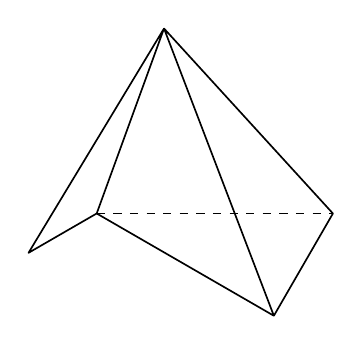
\begin{tikzpicture}[join=round,line width=.6pt,scale=1]
			\path
			(0,0) coordinate (A) ++(0:3) coordinate (B) ++(-120:1.5) coordinate (C)
			(-150:1) coordinate (D) (70:2.5) coordinate (E);
			\draw (A)--(D)--(E)--(A)--(C)--(B)--(E)--(C);
			\draw[dashed] (A)--(B);
			\end{tikzpicture}
			&
			\begin{tikzpicture}[join=round,line width=.6pt,scale=1]
			\path
			(0,0) coordinate (A) ++(120:1.4) coordinate (B) ++(0:2.4) coordinate (C) ++(-60:1.4) coordinate (D)
			($(A)+(0,1.6)$) coordinate (A') ++(120:1.4) coordinate (B') ++(0:2.4) coordinate (C') ++(-60:1.4) coordinate (D')
			($(B')!.25!(C')$) coordinate (M) ($(A')!.55!(D')$) coordinate (N)
			($(M)+(105:1)$) coordinate (A'') ++(.5,0) coordinate (B'') ($(N)-(M)+(B'')$) coordinate (C'')
			++(-.5,0) coordinate (D'');
			\coordinate (P) at (intersection of B'--C' and B''--C'');
			\draw (A)--(A')--(D')--(D)--(A)--(B)--(B')-- (A') (D')--(C')
			(A'')--(B'')--(C'')--(D'')--(A'')--(M)--(N)--(D'')  (N)--(C'') (B')--(M) (P)--(C');
			\draw[dashed] (B)--(C)--(D) (C)--(C') (B'')--(M)--(P);
			\end{tikzpicture}\\
			Hình (1)&Hình (2)&Hình (3)&Hình (4) \vphantom{$ \dfrac{text}{den} $}
		\end{tabular}
	\end{center}
	Mỗi hình trên gồm một số hữu hạn đa giác phẳng (kể cả các điểm trong của nó), hình không phải đa diện là
	\choice
	{Hình $1$}
	{Hình $2$}
	{Hình $3$}
	{\True Hình $4$}
	\loigiai{.}
\end{ex}

\begin{ex}%Câu 4.%[Nguyễn Chiến Thắng, TLDH4]%[2H1B1-2]
	Hình đa diện trong hình vẽ bên có bao nhiêu mặt?
	\begin{center}
		\begin{tikzpicture}[scale=0.7,>=stealth, line join=round, line cap = round]
		\tkzDefPoints{0/0/O, -0.5/.4/A, 1.5/.4/B}
		\coordinate (S) at ($(O)+(0,1.5)$);
		\tkzDefPointBy[symmetry = center O](A) \tkzGetPoint{C}
		\tkzDefPointBy[symmetry = center O](B) \tkzGetPoint{D}
		\tkzDefPointBy[symmetry = center O](S) \tkzGetPoint{S'}
		\tkzDrawSegments[dashed](S,A A,B A,D A,S')
		\tkzDrawSegments(S,B S',D S,C S,D C,D S',B S',C B,C)
		\end{tikzpicture}
	\end{center}
	\choice
	{$8$}
	{\True $10$}
	{$11$}
	{$12$}
	\loigiai{.}
\end{ex}
\begin{ex}%Câu 5.%[Nguyễn Chiến Thắng, TLDH4]%[2H1B1-4]
	Hình lập phương có bao nhiêu mặt phẳng đối xứng?
	\choice
	{$8$}
	{\True $9$}
	{$10$}
	{$12$}
	\loigiai{.}
\end{ex}
\begin{ex}%Câu 6.%[Nguyễn Chiến Thắng, TLDH4]%[2H1B2-1]
	Trong không gian, cho $5$ loại khối đa diện đều như hình vẽ
	\begin{center}
		\begin{tabular}{c c c c c}
			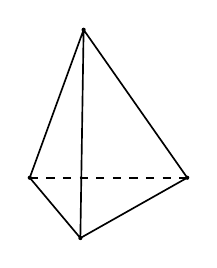
\begin{tikzpicture}[join=round,line width=.6pt,scale=0.5]
			\def\ac{4} % cạnh AC
			\def\ab{2} % cạnh AB
			\def\as{4} % cạnh AS
			\def\gocA{50} % góc A của đáy
			\coordinate[] (A) at (0,0);
			\coordinate[] (C) at (\ac,0);
			\coordinate[] (B) at (-\gocA:\ab);
			\coordinate[] (S) at (70:\as);
			\draw (A)--(B)--(C)--(S)--cycle (S)--(B);
			\draw[dashed] (A)--(C);
			\foreach \diem in {A,B,C,S}\fill (\diem)circle(1.5pt);
			\end{tikzpicture}
			&
			\begin{tikzpicture}[join=round,line width=.5pt,scale=0.5]
			\def\bc{4} % cạnh BC
			\def\ba{2} % cạnh BA
			\def\h{4} % đường cao
			\def\gocB{35} % góc B của đáy
			\coordinate[] (B) at (0,0);
			\coordinate[] (A) at (\gocB:\ba);
			\coordinate[] (C) at (\bc,0);
			\coordinate[] (D) at ($(C)-(B)+(A)$);
			\coordinate[] (A') at ($(A)+(90:\h)$);
			\coordinate[] (B') at ($(B)-(A)+(A')$);
			\coordinate[] (C') at ($(C)-(A)+(A')$);
			\coordinate[] (D') at ($(D)-(A)+(A')$);
			\draw (B')--(B)--(C)--(D)--(D')--(A')--(B')--(C')--(D') (C)--(C');
			\draw[dashed] (A')--(A)--(D) (A)--(B);
			\foreach \diem in {A,B,C,D,A',B',C',D'}	\fill (\diem)circle(1.5pt);
			\end{tikzpicture}
			
			&
			\begin{tikzpicture}[join=round,line width=.5pt,scale=0.5]
			\def\ad{4} % cạnh AD
			\def\ab{2} % cạnh AB
			\def\h{3} % chiều cao trên
			\def\gocA{35} % góc A của đáy hbh
			\coordinate[] (A) at (0,0);
			\coordinate[] (B) at (\gocA:\ab);
			\coordinate[] (D) at (\ad,0);
			\coordinate[] (C) at ($(B)+(D)-(A)$);
			\coordinate (O) at ($(A)!.5!(C)$);
			\coordinate[] (M) at ($(O)+(90:\h)$);
			\coordinate[] (N) at ($(M)!2!(O)$);
			\draw (A)--(D)--(C)--(M)--(A)--(N)--(D)--(M) (N)--(C);
			\draw[dashed] (A)--(B)--(M) (C)--(B)--(N);
			\foreach \diem in {A,B,C,D,M,N}	\fill (\diem)circle(1.5pt);
			\end{tikzpicture}
			&
			\begin{tikzpicture}[join=round,line width=.5pt,scale=0.5]
			\def\R{3} % KC từ tâm đến đỉnh ngoài
			\foreach \x in {0,1,2,...,9}{
				\coordinate (A\x) at (36+\x*36:\R);
				\coordinate (B\x) at ($(0,0)!.7!(A\x)$);}
			\foreach[evaluate=\i as \ki using {int(mod(\i+1,10))}] \i in {0,...,9}\draw (A\i) to (A\ki);
			\foreach \i in {1,3,5,7,9}\draw (B\i)--(A\i);
			\draw (B1)--(B3)--(B5)--(B7)--(B9)--cycle;
			\foreach \i in {0,2,4,6,8}
			\draw[dashed] (B\i)--(A\i);
			\draw[dashed] (B2)--(B4)--(B6)--(B8)--(B0)--cycle;
			\end{tikzpicture}
			&
			\begin{tikzpicture}[join=round,line width=.5pt,scale=0.5]
			\foreach \x in {0,1,2,...,5}{
				\coordinate (A\x) at (-30+\x*60:3);
				\coordinate (B\x) at ($(0,0)!.7!(A\x)$);}
			\foreach[evaluate=\i as \ii using {int(mod(\i+1,6))}] \i in {0,...,5}
			\draw (A\i) to (A\ii);
			\draw[dashed] (B1) edge (A1) edge (A2) edge (A0) edge (B3) edge (B5) (B3) edge (A2) edge (A3) edge (A4) edge (B5) (B5) edge (A4) edge (A5) edge (A0);
			\draw (B0) edge (A0) edge (A1) edge (A5) edge (B2) edge (B4) (B2) edge (A1) edge (A2) edge (A3) edge (B4) (B4) edge (A3) edge (A4) edge (A5);
			\end{tikzpicture}
			\\
			Khối tứ diện đều&Khối lập phương&Bát diện đều&12 mặt đều&20 mặt đều	\vphantom{$ \dfrac{text}{den} $}
		\end{tabular}
	\end{center}
	Mệnh đề nào sau đây đúng?
	\choice
	{Mọi khối đa diện đều có số mặt là những số chia hết cho $4$}
	{\True Khối lập phương và khối bát diện đều có cùng số cạnh}
	{Khối tứ diện đều và khối bát diện đều có $1$ tâm đối xứng}
	{Khối mười hai mặt đều và khối hai mươi mặt đều có cùng số đỉnh}
	\loigiai{.}
\end{ex}
\begin{ex}%Câu 7.%[Nguyễn Chiến Thắng, TLDH4]%[2H1B1-2]
	Cho khối đa diện đều. Khẳng định nào sau đây sai
	\choice
	{Số đỉnh của khối lập phương bằng $8$}
	{Số mặt của khối tứ diện đều bằng $4$}
	{\True Khối bát diện đều là loại $\{4;3\}$}
	{Số cạnh của bát diện đều bằng $12$}
	\loigiai{.}
\end{ex}
\begin{ex}%Câu 8.%[Nguyễn Chiến Thắng, TLDH4]%[2H1B1-2]
	Số đỉnh của một hình bát diện đều là bao nhiêu?
	\choice
	{$10$}
	{$8$}
	{\True $6$}
	{$12$}
	\loigiai{.}
\end{ex}
\begin{ex}%Câu 9.%[Nguyễn Chiến Thắng, TLDH4]%[2H1B1-2]
	Cho đa diện $(H)$ có tất cả các mặt đều là tứ giác. Khẳng định nào sau đây đúng?
	\choice
	{Tổng số các cạnh của $(H)$ luôn bằng tổng số các mặt của $(H)$}
	{Tổng các mặt của $(H)$ luôn bằng tổng số các đỉnh của $(H)$}
	{\True Tổng số các cạnh của $(H)$ luôn là một số chẵn}
	{Tổng số các mặt của $(H)$ luôn là một số lẻ}
	\loigiai{.}
\end{ex}
\begin{ex}%Câu 10.%[Nguyễn Chiến Thắng, TLDH4]%[2H1B3-1]
	Tổng các góc ở đỉnh của tất cả các mặt của khối đa diện đều loại $\{3;5\}$ là
	\choice
	{$12\pi$}
	{$16\pi$}
	{\True $20\pi$}
	{$24\pi$}
	\loigiai{.}
\end{ex}
\begin{ex}%Câu 11.%[Nguyễn Chiến Thắng, TLDH4]%[2H1B3-1]
	Tổng diện tích tất cả các mặt của hình tứ diện đều cạnh $a$ bằng
	\choice
	{$\dfrac{\sqrt{3}a^2}{2}$}
	{$2\sqrt{3}a^2$}
	{\True $\sqrt{3}a^2$}
	{$4\sqrt{3}a^2$}
	\loigiai{
		Tứ diện đều có $4$ mặt là các tam giác đều cạnh $a$ nên tứ diện có tổng diện tích tất cả các mặt là $S=4\cdot\dfrac{\sqrt{3}a^2}{4}=\sqrt{3}a^2$.}
\end{ex}
\begin{ex}%Câu 12.%[Nguyễn Chiến Thắng, TLDH4]%[2H1B3-2]
	Tính thể của hình lập phương có chiều cao $h$ và diện tích đáy là $B$ là
	\choice
	{\True $V=hB$}
	{$V=\dfrac{1}{3}hB$}
	{$V=3hB$}
	{$V=\dfrac{1}{6}hB$}
	\loigiai{.}
\end{ex}

\begin{ex}%Câu 13.%[Nguyễn Chiến Thắng, TLDH4]%[2H1K3-2]
	Cho khối chóp $S.ABCD$ có đáy $ABCD$ là hình chữ nhật, $AB=a$, $AD=a\sqrt{3}$, $SA$ vuông góc với mặt phẳng đáy và mặt phẳng $(SBC)$ tạo với đáy một góc $60^{\circ}$. Tính thể tích $V$ của khối chóp $S.ABCD$.
	\choice
	{$V=3a^3$}
	{$V=\dfrac{\sqrt{3}a^3}{3}$}
	{\True $V=a^3$}
	{$V=\dfrac{a^3}{3}$}
	\loigiai{
		\immini{	Ta có $S_{ABCD}=AB\cdot AD=a\cdot a\sqrt 3=\sqrt 3a^2$.\\
			Dễ thấy $\heva{&BC\perp AB\\&BC\perp SB}\Rightarrow\widehat{SBA}=60^{\circ}$.\\
			Xét tam giác vuông $SAB$ có: $\tan 60^{\circ}=\dfrac{SA}{AB}\Rightarrow SA=AB\tan 60^{\circ}=a\sqrt{3}$.\\
			Vậy $V_{S.ABCD}=\dfrac13 S_{ABCD}\cdot SA=\dfrac13 a^2\sqrt{3}\cdot a\sqrt{3}=a^3$.}
		{
			\begin{tikzpicture}[scale=1, font=\footnotesize, line join=round, line cap=round, >=stealth]
			\def\bc{4} % cạnh BC
			\def\ba{2} % cạnh BA
			\def\h{4} % đường cao
			\def\gocB{30} % góc B của đáy
			\coordinate[label=below left:$D$] (D) at (0,0);
			\coordinate[label=above left:$A$] (A) at (\gocB:\ba);
			\coordinate[label=below:$C$] (C) at (\bc,0);
			\coordinate[label=right:$B$] (B) at ($(C)-(D)+(A)$);
			\coordinate[label=above:$S$] (S) at ($(A)+(90:\h)$);
			\tkzLabelSegments[color=black,pos=.5,above](A,D){a$\sqrt{3}$};
			\tkzLabelSegments[color=black,pos=.5,above](A,B){a}
			\draw (D)--(C)--(B)--(S)--cycle (S)--(C);
			\draw[dashed] (C)--(A)--(B) (S)--(A)--(D)--(B);
			\foreach \diem in {A,B,C,D,S}	\fill (\diem)circle(1.0pt);
			\newcommand{\gocv}[4][black]{\draw[#1] ($(#3)!5pt!(#2)$)--($(#3)!2!($($(#3)!5pt!(#2)$)!.5!($(#3)!5pt!(#4)$)$)$)--($(#3)!5pt!(#4)$);}
			\gocv{S}{A}{D}
			\gocv{S}{A}{B}
			\gocv{B}{A}{D}
			\gocv{S}{B}{C}
			\gocv{S}{D}{C}
			\end{tikzpicture}}
	}
\end{ex}

\begin{ex}%Câu 14.%[Nguyễn Chiến Thắng, TLDH4]%[2H1K3-2]
	Cho hình chóp tam giác $S.ABC$ có đáy $ABC$ là tam giác vuông tại $A$, $AB=a$, $AC=2a$, cạnh bên $SA$ vuông góc với mặt đáy và $SA=a$. Tính thể tích $V$ của khối chóp $S.ABC$.
	\choice
	{$V=a^3$}
	{$V=\dfrac{a^3}{2}$}
	{\True $V=\dfrac{a^3}{3}$}
	{$V=\dfrac{a^3}{4}$}
	\loigiai{
		\immini{	Diện tích đáy $B=S_{ABC}=\dfrac{1}{2}a\cdot 2a=a^2$.\\
			Chiều cao: $h=a$.\\
			$V_{ABCA’B’C’}=\dfrac{1}{3}B\cdot h=\dfrac{1}{3}a^2\cdot a=\dfrac{a^3}{3}$.}
		{
			\begin{tikzpicture}[scale=1, font=\footnotesize, line join=round, line cap=round, >=stealth]
			\def\ac{4} % cạnh AC
			\def\ab{2} % cạnh AB
			\def\h{4} % chiều cao
			\def\gocA{50} % góc A của đáy
			\coordinate[label=left:$A$] (A) at (0,0);
			\coordinate[label=right:$C$] (C) at (\ac,0);
			\coordinate[label=below left:$B$] (B) at (-\gocA:\ab);
			\coordinate[label=above:$S$] (S) at ($(A)+(90:\h)$);
			\tkzLabelSegments[color=black,pos=.5,left](A,S){a}
			\tkzLabelSegments[color=black,pos=.5,left](A,B){a}
			\tkzLabelSegments[color=black,pos=.5,above](A,C){2a}
			\draw (A)--(B)--(C)--(S)--cycle (S)--(B);
			\draw[dashed] (A)--(C);
			\foreach \diem in {A,B,C,S}	\fill (\diem)circle(1.5pt);
			\newcommand{\gocv}[4][black]{\draw[#1] ($(#3)!5pt!(#2)$)--($(#3)!2!($($(#3)!5pt!(#2)$)!.5!($(#3)!5pt!(#4)$)$)$)--($(#3)!5pt!(#4)$);}
			\gocv{S}{A}{C}
			\end{tikzpicture}}
	}
\end{ex}
\begin{ex}%Câu 15.%[Nguyễn Chiến Thắng, TLDH4]%[2H1K3-2]
	Cho hình chóp tứ giác đều có tất cả các cạnh bằng nhau, đường cao của một mặt bên là $a\sqrt{3}$. Thể tích $V$ của khối chóp đó là
	\choice
	{$V=\dfrac{2\sqrt{2}}{3}a^3$}
	{\True $V=\dfrac{4\sqrt{2}}{3}a^3$}
	{$V=\dfrac{\sqrt{2}}{6}a^3$}
	{$V=\dfrac{\sqrt{2}}{9}a^3$}
	\loigiai{
		\immini{Ta có $SM=a\sqrt{3}$. $\Delta SCD$ đều nên $SC=CD=2a$.\\
			Suy ra: $SO=\dfrac{AC}{2}=\dfrac{2a\sqrt{2}}{2}=a\sqrt{2}$.\\
			Vậy $V=\dfrac{1}{3}SO\cdot S_{ABCD}=\dfrac{1}{3}a\sqrt{2}\cdot 4a^2=\dfrac{4a^3\sqrt{2}}{3}$.}
		{
			\begin{tikzpicture}[scale=1, font=\footnotesize, line join=round, line cap=round, >=stealth]
			\def\bc{4} % cạnh BC
			\def\ba{2} % cạnh BA
			\def\h{4} % đường cao
			\def\gocB{30} % góc B của đáy
			\coordinate[label=below left:$B$] (B) at (0,0);
			\coordinate[label=above right:$A$] (A) at (\gocB:\ba);
			\coordinate[label=below:$C$] (C) at (\bc,0);
			\coordinate[label=right:$D$] (D) at ($(C)-(B)+(A)$);
			\coordinate[label=below:$O$] (O) at ($(A)!.5!(C)$);
			\coordinate[label=above:$S$] (S) at ($(O)+(90:\h)$);
			\tkzDefMidPoint(C,D) \tkzGetPoint{M};
			\tkzLabelPoints[below right,color=black](M)
			\draw (B)--(C)--(D)--(S)--cycle (S)--(C) (S)--(M);
			\draw[dashed] (C)--(A)--(D)--(B) (M)--(O)--(S)--(A)--(B);
			\foreach \diem in {A,B,C,D,S,O,M}	\fill (\diem)circle(1.5pt);
			\end{tikzpicture}}
	}
\end{ex}
\begin{ex}%Câu 16.%[Nguyễn Chiến Thắng, TLDH4]%[2H1K3-2]
	Cho khối chóp $S.ABCD$ có đáy $ABCD$ là hình vuông cạnh $a$, cạnh bên $SA$ vuông góc với mặt phẳng đáy,góc giữa mặt phẳng $(SBD)$ và mặt phẳng đáy bằng $60^{\circ}$. Tính thể tích $V$ của khối chóp $S.ABCD$.
	\choice
	{\True $V=\dfrac{a^3\sqrt{6}}{6}$}
	{$V=\dfrac{a^3\sqrt{3}}{2}$}
	{$V=\dfrac{a^3\sqrt{3}}{12}$}
	{$V=\dfrac{a^3\sqrt{3}}{7}$}
	\loigiai{
		\immini{Ta có $S_{ABCD}=a^2$.\\
			$SA=AO\cdot\tan\widehat{SOA}=\dfrac{a\sqrt{2}}{2}\cdot\tan 60^{\circ}=\dfrac{a\sqrt{6}}{2}$,\\ $V_{S\cdot ABCD}=\dfrac 13\cdot S_{ABCD}\cdot SA=\dfrac{a^3\sqrt 6}6$.}
		{
			\begin{tikzpicture}[scale=1, font=\footnotesize, line join=round, line cap=round, >=stealth]
			\def\bc{4} % cạnh BC
			\def\ba{2} % cạnh BA
			\def\h{4} % đường cao
			\def\gocB{30} % góc B của đáy
			\coordinate[label=below left:$B$] (B) at (0,0);
			\coordinate[label=above right:$A$] (A) at (\gocB:\ba);
			\coordinate[label=below:$C$] (C) at (\bc,0);
			\coordinate[label=right:$D$] (D) at ($(C)-(B)+(A)$);
			\coordinate[label=below:$O$] (O) at ($(A)!.5!(C)$);
			\coordinate[label=above:$S$] (S) at ($(O)+(90:\h)$);
			\draw (B)--(C)--(D)--(S)--cycle (S)--(C);
			\draw[dashed] (C)--(A)--(D)--(B) (O)--(S)--(A)--(B);
			\foreach \diem in {A,B,C,D,S}	\fill (\diem)circle(1.5pt);
			\end{tikzpicture}}
	}
\end{ex}
\begin{ex}%Câu 17.%[Nguyễn Chiến Thắng, TLDH4]%[2H1K3-2]
	Cho hình chóp $S.ABC$ có $SAB$ và $ABC$ là hai tam giác đều và nằm trong hai mặt phẳng vuông góc với nhau, $SC=\dfrac{a\sqrt{6}}{2}$. Tính thể tích $V$ của khối chóp $S.ABC$.
	\choice
	{$V=\dfrac{a^3}{12}$}
	{$V=\dfrac{a^3}{4}$}
	{$V=\dfrac{3a^3}{8}$}
	{\True $V=\dfrac{a^3}{8}$}
	\loigiai{
		\immini{Gọi $I$ là trung điểm của $AB$ ta có $AB\perp(SIC)$. Mặt khác, góc giữa hai mặt phẳng $(SAB)$ và $(ABC)$ là góc $\widehat{SIC}=90^{\circ}\Rightarrow SI\perp(ABC)$.\\
			Đặt $AB=x\Rightarrow SI=CI=\dfrac{x\sqrt{3}}{2}\Rightarrow\dfrac{x\sqrt{3}}{2}\cdot\sqrt{2}=\dfrac{a\sqrt{6}}{2}\Rightarrow x=a$.\\
			Vậy thể tích tứ diện là $V_{S.ABC}=\dfrac{1}{3}\cdot\dfrac{a\sqrt{3}}{2}\cdot\dfrac{a^2\sqrt{3}}{4}=\dfrac{a^3}{8}$.}
		{
			\begin{tikzpicture}[scale=1, font=\footnotesize, line join=round, line cap=round, >=stealth]
			\def\ac{4} % cạnh AC
			\def\ab{3} % cạnh AB
			\def\h{5} % chiều cao
			\def\gocA{30} % góc A của đáy
			\coordinate[label=left:$A$] (A) at (0,0);
			\coordinate[label=right:$C$] (C) at (\ac,0);
			\coordinate[label=below:$B$] (B) at (-\gocA:\ab);
			\coordinate[label=below left:$I$] (I) at ($(A)!.5!(B)$);
			\coordinate[label=above:$S$] (S) at ($(I)+(90:\h)$);
			\tkzLabelSegments[color=black,pos=.5,above](S,C){$\dfrac{a\sqrt{6}}{2}$};
			\draw (A)--(B)--(C)--(S)--cycle (I)--(S)--(B);
			\draw[dashed] (A)--(C)--(I);
			\foreach \diem in {A,B,C,S,I}	\fill (\diem)circle(1.0pt);
			\newcommand{\gocv}[4][black]{\draw[#1] ($(#3)!5pt!(#2)$)--($(#3)!2!($($(#3)!5pt!(#2)$)!.5!($(#3)!5pt!(#4)$)$)$)--($(#3)!5pt!(#4)$);}
			\gocv{S}{I}{A}
			\gocv{S}{I}{C}
			\gocv{C}{I}{A}
			\end{tikzpicture}}
	}
\end{ex}
\begin{ex}%Câu 18.%[Nguyễn Chiến Thắng, TLDH4]%[2H1K3-2]
	Cho hình chóp $S.ABC$ có đáy $ABC$ là tam giác vuông cân tại $B$, có $BC=a$. Mặt bên $(SAC)$ vuông góc với đáy, các mặt bên còn lại đều tạo với mặt đáy một góc $45^{\circ}$. Tính thể tích khối chóp $SABC$.
	\choice
	{\True $\dfrac{a^3}{12}$}
	{$a^3$}
	{$\dfrac{a^3}{6}$}
	{$\dfrac{a^3}{24}$}
	\loigiai{
		\immini{	Gọi $H$ là hình chiếu vuông góc của $S$ lên cạnh $AC$ nên $SH\perp(ABC)$.\\
			Gọi $E$, $F$ lần lượt là hình chiếu vuông góc của $H$ lên cạnh $AB$ và $AC$. Khi đó, góc tạo bởi hai mặt phẳng $(SAB)$, $(SAC)$ tạo với đáy lần lượt là $\widehat{SEH}$, $\widehat{SFH}$ cùng bằng $45^{\circ}$.\\
			Hai tam giác $\Delta SEH$, $\Delta SFH$ có $\widehat{SHE}=\widehat{SHF}=90^{\circ}$, $SH$ chung, $\widehat{HSE}=\widehat{HSF}=45^{\circ}$ nên hai tam giác bằng nhau hay $HE=HF$. Mà $\Delta ABC$ là tam giác vuông cân nên $H$ là trung điểm của $AC$.\\
			Ta có: $SH=HE=\dfrac{BC}{2}=\dfrac{a}{2}$. \\
			Vậy $V_{S.ABC}=\dfrac{1}{3}S_{ABC}\cdot SH=\dfrac{1}{3}\cdot\dfrac{a^2}{2}\cdot\dfrac{a}{2}=\dfrac{a^3}{12}$.}
		{	\begin{tikzpicture}[scale=1, font=\footnotesize, line join=round, line cap=round, >=stealth]
			\def\ac{4} % cạnh AC
			\def\ab{3} % cạnh AB
			\def\h{5} % chiều cao
			\def\gocA{30} % góc A của đáy
			\coordinate[label=left:$A$] (A) at (0,0);
			\coordinate[label=right:$B$] (B) at (\ac,0);
			\coordinate[label=below:$C$] (C) at (-\gocA:\ab);
			\coordinate[label=below left:$H$] (H) at ($(A)!.5!(C)$); % Thay đổi số 1/2 để đổi vị trí điểm H
			\coordinate[label=above:$S$] (S) at ($(H)+(90:\h)$);
			\tkzDefMidPoint(A,B) \tkzGetPoint{E}
			\tkzDefMidPoint(C,B) \tkzGetPoint{F}
			\tkzLabelPoints[right,color=black](F)
			\tkzLabelPoints[above left,color=black](E)
			\draw (A)--(C)--(B)--(S)--cycle (H)--(S)--(C) (S)--(F);
			\draw[dashed] (A)--(B) (S)--(E)--(H)--(F);
			\foreach \diem in {A,B,C,S,H,E,F}	\fill (\diem)circle(1.0pt);
			\end{tikzpicture}}
	}
\end{ex}
\begin{ex}%Câu 19.%[Nguyễn Chiến Thắng, TLDH4]%[2H1K3-2]
	Cho hình chóp tam giác đều có cạnh đáy bằng $a$ và cạnh bên bằng $b$. Thể tích của khối chóp là
	\choice
	{$\dfrac{a^2}{4}\sqrt{3b^2-a^2}$}
	{\True $\dfrac{a^2}{12}\sqrt{3b^2-a^2}$}
	{$\dfrac{a^2}{6}\sqrt{3b^2-a^2}$}
	{$a^2\sqrt{3b^2-a^2}$ }
	\loigiai{
		Gọi $S.ABC$ là hình chóp tam giác đều và $G$ là trọng tâm tam giác $ABC$. Khi đó, $SG\perp(ABC)$ và $AB=a$, $SB=b$, $AG=\dfrac{2}{3}\cdot\dfrac{a\sqrt{3}}{2}=\dfrac{a\sqrt{3}}{3}\Rightarrow SG=\sqrt{SA^2-AG^2}=\sqrt{\dfrac{3b^2-a^2}{3}}$.\\
		Vậy $V_{S.ABC}=\dfrac{1}{3}SG\cdot S_{\triangle ABC}=\dfrac{1}{3}\cdot\dfrac{a^2\sqrt{3}}{4}\cdot\sqrt{\dfrac{3b^2-a^2}{3}}=\dfrac{a^2}{12}\sqrt{3b^2-a^2}$.}
\end{ex}
\begin{ex}%Câu 20.%[Nguyễn Chiến Thắng, TLDH4]%[2H1K3-3]
	Cho hình chóp tam giác $S.ABC$ có $M$ là trung điểm $SB$, $N$ là điểm trên $SC$ sao cho $NS=2NC$, là điểm trên $SA$ sao cho $PA=2PS$. Kí hiệu $V_1$, $V_2$ lần lượt là thể tích khối chóp $BMNP$ và $S.ABC$. Tính tỉ số $\dfrac{V_1}{V_2}$.
	\choice
	{\True $\dfrac{V_1}{V_2}=\dfrac{1}{9}$}
	{$\dfrac{V_1}{V_2}=\dfrac{3}{4}$}
	{$\dfrac{V_1}{V_2}=\dfrac{2}{3}$}
	{$\dfrac{V_1}{V_2}=\dfrac{1}{3}$}
	\loigiai{
		\immini{$\dfrac{V_{N.BMP}}{V_{C.SAB}}=\dfrac{\dfrac{1}{3}\mathrm{d}\left(N,(SAB)\right)\cdot S_{BMP}}{\dfrac{1}{3}\mathrm{d}\left(C,(SAB)\right)\cdot S_{SAB}}$;\\
			$\dfrac{\mathrm{d}\left(N,(SAB)\right)}{\mathrm{d}\left(C,(SAB)\right)}=\dfrac{NS}{CS}=\dfrac{2}{3}$;\\
			$S_{SBM}=\dfrac{1}{2}S_{BPS}=\dfrac{1}{2}\cdot\dfrac{1}{3}\cdot S_{SAB}\Rightarrow\dfrac{V_{N.BMP}}{V_{C.SAB}}=\dfrac{2}{3}\cdot\dfrac{1}{6}=\dfrac{1}{9}$.}
		{\begin{tikzpicture}[scale=1, font=\footnotesize, line join=round, line cap=round, >=stealth]
			\def\ac{4} % cạnh AC
			\def\ab{2} % cạnh AB
			\def\as{4} % cạnh AS
			\def\gocA{50} % góc A của đáy
			\coordinate[label=left:$A$] (A) at (0,0);
			\coordinate[label=right:$C$] (C) at (\ac,0);
			\coordinate[label=below:$B$] (B) at (-\gocA:\ab);
			\coordinate[label=above:$S$] (S) at (70:\as);
			\tkzDefMidPoint(S,B) \tkzGetPoint{M};
			\tkzDefPointBy[homothety = center S ratio 2/3](C) \tkzGetPoint{N}
			\tkzDefPointBy[homothety = center S ratio 1/3](A) \tkzGetPoint{P}
			\tkzLabelPoints[left,color=black](P)
			\tkzLabelPoints[above right,color=black](M,N)
			\draw (A)--(B)--(C)--(S)--cycle (P)--(B)--(S)--(C) (P)--(M)--(N);
			\draw[dashed] (N)--(P) (A)--(C);
			\foreach \diem in {A,B,C,S,M,N,P}\fill (\diem)circle(1.0pt);
			\end{tikzpicture}}
	}
\end{ex}
\begin{ex}%Câu 21.%[Nguyễn Chiến Thắng, TLDH4]%[2H1K3-6]
	Một khối hộp chữ nhật $ABCD.A_1B_1C_1D_1$ có đáy $ABCD$ là một hình vuông. Biết tổng diện tích tất cả các mặt của khối hộp đó là $32$, thể tích lớn nhất mà khối hộp $ABCD.A_1B_1C_1D_1$ đạt được là bao nhiêu?
	\choice
	{$\dfrac{56\sqrt{3}}{9}$}
	{$\dfrac{80\sqrt{3}}{9}$}
	{$\dfrac{70\sqrt{3}}{9}$}
	{\True $\dfrac{64\sqrt{3}}{9}$}
	\loigiai{
		Đặt $a$ là độ dài cạnh của hình vuông đáy, $b$ là chiều cao của khối hộp với $a$, $b>0$.\\
		Theo đề bài, ta có $2a^2+4ab=32\Leftrightarrow 2a(a+2b)=32\Leftrightarrow a(a+2b)=16\Leftrightarrow b=\dfrac{1}{2}\left(\dfrac{16}{a}-a\right)$.\\
		Khi đó thể tích của khối hộp $V=a^2\cdot\dfrac{1}{2}\left(\dfrac{16}{a}-a\right)=-\dfrac{1}{2}a^3+8a$.\\
		Khảo sát hàm $f(a)=-\dfrac{1}{2}a^3+8a$ với $a>0$, ta được $\max\limits_{(0;+\infty)} f(a)=f\left(\dfrac{4}{\sqrt{3}}\right)=\dfrac{64\sqrt{3}}{9}$.}
\end{ex}
\begin{ex}%Câu 22.%[Nguyễn Chiến Thắng, TLDH4]%[2H1K3-3]
	Cho hình chóp đều $S.ABCD$. Gọi $N$ là trung điểm $SB, M$ là điểm đối xứng với $B$ qua $A$. Mặt phẳng $(MNC)$ chia khối chóp $S.ABCD$ thành hai phần có thể tích lần lượt là $V_1, V_2$ với $V_1<V_2$. Tính tỉ số $\dfrac{V_1}{V_2}$.
	\choice
	{\True $\dfrac{V_1}{V_2}=\dfrac{5}{7}$}
	{$\dfrac{V_1}{V_2}=\dfrac{5}{11}$}
	{$\dfrac{V_1}{V_2}=\dfrac{5}{9}$}
	{$\dfrac{V_1}{V_2}=\dfrac{5}{13}$}
	\loigiai{
		\immini{	Gọi $h$, $S$ lần lượt là chiều cao và diện tích đáy của khối chóp $S.ABCD$. Khi đó $V_{S.ABCD}=\dfrac{1}{3}S\cdot h$. Nối $MN$ cắt $SA$ tại $E$, $MC$ cắt $AD$ tại $F$. Tam giác $SBM$ có $A$, $N$ lần lượt là trung điểm của $BM$ và $SB$ suy ra $E$ là trọng tâm tam giác $SBM$. Tứ giác $ACDM$ là hình bình hành nên $F$ là trung điểm $MC$.\\
			Ta có $V_{BNC\cdot AEF}=V_{ABCEN}+V_{E.ACF}$.\\
			$\dfrac{V_{S.ENC}}{V_{S.ABC}}=\dfrac{SE}{SA}\cdot\dfrac{SN}{SB}=\dfrac{2}{3}\cdot\dfrac{1}{2}=\dfrac{1}{3}$\\
			$\Rightarrow V_{S.ENC}=\dfrac{1}{3}V_{S.ABC}$.\\
		}
		{
			\begin{tikzpicture}[scale=1, font=\footnotesize, line join=round, line cap=round, >=stealth]
			\def\bc{4} % cạnh BC
			\def\ba{2} % cạnh BA
			\def\h{4} % đường cao
			\def\gocB{30} % góc B của đáy
			\coordinate[label=below left:$D$] (D) at (0,0);
			\coordinate[label=above right:$A$] (A) at (\gocB:\ba);
			\coordinate[label=below:$C$] (C) at (\bc,0);
			\coordinate[label=right:$B$] (B) at ($(C)-(D)+(A)$);
			\coordinate[label=above right:$O$] (O) at ($(A)!.5!(C)$);
			\coordinate[label=above:$S$] (S) at ($(O)+(90:\h)$);
			\tkzDefPointBy[symmetry = center A](B) \tkzGetPoint{M};
			\tkzLabelPoints[above left,color=black](M)
			\tkzDefMidPoint(S,B) \tkzGetPoint{N};
			\tkzLabelPoints[above right,color=black](N)
			\tkzDefMidPoint(A,D) \tkzGetPoint{F};
			\tkzLabelPoints[above,color=black](F)
			\tkzInterLL(M,N)(S,A) \tkzGetPoint{E};
			\tkzLabelPoints[above left,color=black](E)
			\tkzInterLL(M,C)(S,D) \tkzGetPoint{R};
			\tkzInterLL(M,N)(S,D) \tkzGetPoint{T};
			
			\draw (D)--(C)--(B)--(S)--cycle (S)--(C)--(N) (R)--(M)--(T);
			\draw[dashed] (C)--(A)--(B)--(D) (O)--(S)--(A)--(D) (M)--(A) (C)--(F)--(E)--(N) (R)--(F) (T)--(E);
			\foreach \diem in {A,B,C,D,S,O,M,N,E,F}	\fill (\diem)circle(1.0pt);
			\end{tikzpicture}}
		\noindent
		$\Rightarrow V_{ABCEN}=\dfrac{2}{3}V_{S.ABC}=\dfrac{2}{3}\left(\dfrac{1}{2}V_{S.ABCD}\right)=\dfrac{1}{3}V_{S.ABCD}$.\\
		$V_{E.ACF}=\dfrac{1}{3}S_{\triangle ACF}\cdot \mathrm{d}[E,(ACF)]=\dfrac{1}{3}\cdot\dfrac{1}{4}S\cdot\dfrac{1}{3}h=\dfrac{1}{12}V_{S.ABCD}$.\\
		Do đó, $V_{BNC\cdot AEF}=V_{ABCEN}+V_{E.ACF}=\dfrac{1}{3}V_{S.ABCD}+\dfrac{1}{12}V_{S.ABCD}=\dfrac{5}{12}V_{S.ABCD}=V_1$.\\
		Suy ra $V_2=\dfrac{7}{12}V_{S.ABCD}\Rightarrow\dfrac{V_1}{V_2}=\dfrac{5}{7}$.
	}
\end{ex}
\begin{ex}%Câu 23.%[Nguyễn Chiến Thắng, TLDH4]%[2H1K3-2]
	Cho khối chóp $S.ABC$ có đường cao $SA=2a$, tam giác $ABC$ vuông ở $C$ có $AB=2a$, góc $\widehat{CAB}=30^{\circ}$. Gọi $H$ là hình chiếu của $A$ trên $SC$. Gọi $B’$ là điểm đối xứng của $B$ qua mặt phẳng $(SAC)$. Tính thể tích khối chóp $H.AB’B$
	\choice
	{\True $\dfrac{2a^3\sqrt{3}}{7}$}
	{$\dfrac{2a^3\sqrt{3}}{7}$}
	{$\dfrac{6a^3\sqrt{3}}{7}$}
	{$\dfrac{a^3\sqrt{3}}{7}$}
	\loigiai{
		\immini{	Ta có: $AC=AB\cos C=a\sqrt{3};BC=a;S_{ABC}=\dfrac{a^3\sqrt{3}}{2}$.\\
			Lại có $SA^2=SH\cdot SC\Rightarrow\dfrac{SH}{SC}=\dfrac{SA^2}{SC^2}=\dfrac{SA^2}{SA^2+AC^2}=\dfrac{4}{7}$.\\
			Do đó $\mathrm{d}\left(H;(ABC)\right)=\dfrac{3}{7}SA=\dfrac{6}{7}a;S_{ABB’}=2S_{ABC}=a^2\sqrt{3}$.\\
			Suy ra $V_{H.ABB’}=\dfrac{2a^3\sqrt{3}}{7}$.}
		{
			\begin{tikzpicture}[scale=1, font=\footnotesize, line join=round, line cap=round, >=stealth]
			\def\ac{4} % cạnh AC
			\def\ab{3} % cạnh AB
			\def\h{4} % chiều cao
			\def\gocA{40} % góc A của đáy
			\coordinate[label=left:$A$] (A) at (0,0);
			\coordinate[label=right:$B$] (B) at (\ac,0);
			\coordinate[label=below right:$C$] (C) at (-\gocA:\ab);
			\coordinate[label=above:$S$] (S) at ($(A)+(90:\h)$);
			\tkzDefPointBy[symmetry = center C](B) \tkzGetPoint{B'};
			\tkzLabelPoints[left,color=black](B')
			\tkzDefPointBy[homothety = center S ratio 1/3](C) \tkzGetPoint{H}
			\tkzLabelPoints[left,color=black](H)
			\draw (C)--(B)--(S)--cycle (S)--(C)--(B')--(A)--(S) (A)--(H)--(B') (H)--(B);
			\draw[dashed] (C)--(A)--(B) (B')--(A);
			\foreach \diem in {A,B,C,S,B',H}	\fill (\diem)circle(1.0pt);
			\newcommand{\gocv}[4][black]{\draw[#1] ($(#3)!5pt!(#2)$)--($(#3)!2!($($(#3)!5pt!(#2)$)!.5!($(#3)!5pt!(#4)$)$)$)--($(#3)!5pt!(#4)$);}
			\gocv{S}{A}{C}
			\gocv{S}{A}{B}
			\gocv{A}{C}{B}
			\end{tikzpicture}}
	}
\end{ex}
\begin{ex}%Câu 24.%[Nguyễn Chiến Thắng, TLDH4]%[2H1K3-2]
	Cho hình chóp $S.ABCD$ có đáy $ABCD$ là hình thang vuông tại $A$ và $B$, $BA=BC=1$, $AD=2$. Cạnh bên $SA$ vuông góc với đáy và $SA=\sqrt{2}$. Gọi $H$ là hình chiếu vuông góc của $V=a^3$ trên $SB$. Tính thể tích $V$ của khối đa diện $SAHCD$.
	\choice
	{$V=\dfrac{2\sqrt{2}}{3}$}
	{\True $V=\dfrac{4\sqrt{2}}{9}$}
	{$V=\dfrac{4\sqrt{2}}{3}$}
	{$V=\dfrac{2\sqrt{2}}{9}$}
	\loigiai{
		\immini{	Tam giác vuông $SAB$, có $SB=\sqrt{SA^2+AB^2}=\sqrt{3}$.\\
			Gọi $M$ là trung điểm $AD\Rightarrow ABCM$ là hình vuông nên $CM=AB=a=\dfrac{AD}{2}$.\\
			$\Rightarrow$ tam giác $ACD$ vuông tại $C$.\\
			Ta có $V_{S.AHCD}=V_{S.ACD}+V_{S.AHC}$.\\
			$V_{S.ACD}=\dfrac{1}{3}S_{\triangle ACD}\cdot SA=\dfrac{1}{3}\left(\dfrac{1}{2}AD\cdot AB\right)SA=\dfrac{\sqrt{2}}{3}$.\\
			$\dfrac{V_{S.AHC}}{V_{S.ABC}}=\dfrac{SH}{SB}=\dfrac{SA^2}{SB^2}=\dfrac{2}{3}\Rightarrow V_{S.AHC}=\dfrac{2}{3}V_{S.ABC}=\dfrac{\sqrt{2}}{9}$.\\
			Vậy $V_{S.AHCD}=\dfrac{\sqrt{2}}{3}+\dfrac{\sqrt{2}}{9}=\dfrac{4\sqrt{2}}{9}$.}
		{
			\begin{tikzpicture}[scale=1, font=\footnotesize, line join=round, line cap=round, >=stealth]
			\def\bc{4} % cạnh BC
			\def\ba{2} % cạnh BA
			\def\h{5} % đường cao
			\def\gocB{30} % góc B của đáy
			\coordinate[label=below left:$B$] (B) at (0,0);
			\coordinate[label=below:$A$] (A) at (\gocB:\ba);
			\coordinate[label=below:$C$] (C) at (\bc,0);
			\coordinate[] (E) at ($(C)-(B)+(A)$);
			\tkzDefPointBy[homothety = center A ratio 1.3](E) \tkzGetPoint{D};
			\tkzLabelPoints[right,color=black](D)
			\coordinate[label=above:$S$] (S) at ($(A)+(90:\h)$);
			\tkzDefMidPoint(A,D) \tkzGetPoint{M}
			\tkzLabelPoints[above,color=black](M)
			\tkzDefPointBy[homothety = center S ratio 2/3](B) \tkzGetPoint{H}
			\tkzLabelPoints[above left,color=black](H)
			\draw (B)--(C)--(D)--(S)--cycle (S)--(C)--(H);
			\draw[dashed] (M)--(C)--(A)--(D) (S)--(A)--(B) (H)--(A);
			\foreach \diem in {A,B,C,D,S,M}	\fill (\diem)circle(1.0pt);
			\newcommand{\gocv}[4][black]{\draw[#1] ($(#3)!5pt!(#2)$)--($(#3)!2!($($(#3)!5pt!(#2)$)!.5!($(#3)!5pt!(#4)$)$)$)--($(#3)!5pt!(#4)$);}
			\gocv{S}{A}{D}
			\end{tikzpicture}}
	}
\end{ex}
\begin{ex}%Câu 25.%[Nguyễn Chiến Thắng, TLDH4]%[2H1K3-6]
	\immini{	Người ta cắt một tờ giấy hình vuông cạnh bằng $1$ để gấp thành một hình chóp tứ giác đều sao cho bốn đỉnh của hình vuông dán lại thành đỉnh của hình chóp (hình vẽ). Để thể tích khối chóp lớn nhất thì cạnh đáy $x$ của hình chóp bằng}
	{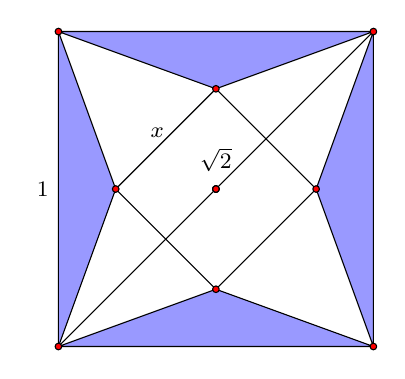
\begin{tikzpicture}[line join=round,scale=4,font=\footnotesize]
		\def\a{1}\def\x{.45}
		\draw (-\a/2,-\a/2)--(\a/2,\a/2);
		\foreach \i in {0,90,180,270}{
			\begin{scope}[rotate=\i]
			\draw[fill=blue!40] (0,0) (0,{-\x*sqrt(2)/2})--({\x*sqrt(2)/2},0)--(\a/2,\a/2)--(\a/2,-\a/2)--({\x*sqrt(2)/2},0);
			\end{scope}};
		\foreach \i in {0,90,180,270}{
			\begin{scope}[rotate=\i]
			\draw[fill=red](0,0)circle (.3pt) ({\x*sqrt(2)/2},0)circle (.3pt) (\a/2,\a/2)circle (.3pt);
			\end{scope}};
		\path (0,0)node[above=1mm]{$ \sqrt{2} $} (-\a/2,0)node[left]{$ 1 $} ({-\x*sqrt(2)/4},{\x*sqrt(2)/4})node[above left=-1mm]{$ x $};
		\end{tikzpicture}}
	\choice
	{$x=\dfrac{\sqrt{2}}{5}$}
	{\True $x=\dfrac{2\sqrt{2}}{5}$}
	{$x=2\sqrt{2}$}
	{$x=\dfrac{2}{5}$}
	\loigiai{
		Ta có $BM=\dfrac{1}{2}AB-MO=\dfrac{\sqrt{2}}{2}-\dfrac{x}{2}$.\\
		Chiều cao của hình chóp:\\
		$h=\sqrt{BM^2-MO^2}=\sqrt{\left(\dfrac{\sqrt{2}}{2}-\dfrac{x}{2}\right)^2-\left(\dfrac{x}{2}\right)^2}=\sqrt{\dfrac{1-x\sqrt{2}}{2}}$.\\
		Thể tích của khối chóp $V=\dfrac{1}{3}x^2\sqrt{\dfrac{1-x\sqrt{2}}{2}}=\dfrac{1}{3}\sqrt{\dfrac{x^4-x^5\sqrt{2}}{2}}$.\\
		Khảo sát hàm số $f(x)=x^4-x^5\sqrt 2$ trên $\left(0;\dfrac{\sqrt 2}2\right)$, ta được GTLN của hàm số đạt tại $x=\dfrac{2\sqrt 2}5$.}
\end{ex}
\Closesolutionfile{ans}
\DAPAN
\inputansbox	{10}{ans/ans-2H1-5KT1-2} 